% Leonardo BMC Bioinformatics draft.
% Template: Springer Nature LaTeX authoring template, December 2024.
\documentclass[pdflatex,sn-vancouver-num]{sn-jnl}

\usepackage{graphicx}
\usepackage{booktabs}
\usepackage{array}
\usepackage{amsmath,amssymb}
\usepackage{tabularx}
\usepackage{xurl}
\usepackage{placeins}

\raggedbottom

\begin{document}

\title[Leonardo structural bioinformatics workflows]{Leonardo: an integrated PyMOL-based platform for structural bioinformatics workflow orchestration and verification}

\author*[1,2]{\fnm{Juvenal} \sur{Yosa}}\email{jyosa@protyon.tech}
\author[3]{\fnm{Matthew R.} \sur{Groves}}
\author[2]{\fnm{Anthonie J.} \sur{van der Wekken}}

\affil*[1]{\orgname{Protyon Tech}, \orgaddress{\country{Colombia}}}
\affil[2]{\orgname{University Medical Center Groningen}, \orgaddress{\city{Groningen}, \country{The Netherlands}}}
\affil[3]{\orgdiv{Chemical and Pharmaceutical Biology, Groningen Research Institute of Pharmacy}, \orgname{University of Groningen}, \orgaddress{\city{Groningen}, \country{The Netherlands}}}

\abstract{\textbf{Background:} Structural bioinformatics increasingly combines sequence annotation, experimental or predicted structures, ligand preparation, docking, molecular dynamics diagnostics and quantum chemistry.  These steps are usually distributed across command-line programs, notebooks and molecular viewers, creating a barrier for experimental or interdisciplinary users who need repeatable computational experiments but do not necessarily have computational-specialist training.
\textbf{Results:} We present Leonardo, a modular PyMOL-based application that organizes these tasks into project-aware workflows.  Leonardo distinguishes adapter modules that expose established tools from native workflow pipelines that add object mapping, workflow checks, repeated sampling and reaction-path construction.  The architecture covers 15 modules and more than 30 cited external tool or service dependencies.  Representative module-level examples exercise protein-ligand contact reporting, fpocket/smina pocket-to-grid handoff, single-target template redocking, ligand-library quality control, OpenMM collective-variable setup, guided-exit binding diagnostics and Psi4/MOPAC reaction-path orchestration.  These examples document that Leonardo can prepare inputs, preserve object provenance, execute or parse external engines, generate PyMOL-linked reports and rebuild manuscript figures from traceable source artifacts.  The software verification suite completed with 524 passing tests in the declared \texttt{protliginteract-full} environment.  The reported examples are workflow-verification cases rather than general benchmarks of docking, virtual-screening enrichment, production binding free energies, force-field accuracy or transition-state energetics.
\textbf{Conclusions:} Leonardo is designed to reduce manual handoffs between biological inputs and physics-based or cheminformatics analyses while keeping specialized algorithms transparently cited and externally replaceable.  Its contribution is a reproducible structural bioinformatics workflow layer rather than a replacement for established scientific engines.}

\keywords{structural bioinformatics, protein-ligand interactions, molecular docking, molecular dynamics, PyMOL, workflow software}

\maketitle

\section{Background}\label{sec:background}

Protein structure analysis has moved from a specialist computational activity to a routine part of many biological projects.  Experimental structures, AlphaFold models, mutagenesis hypotheses, ligand libraries, enzymatic mechanisms and molecular-dynamics trajectories are now commonly interpreted together.  A single study may begin with sequence retrieval and motif interpretation, continue through homology modeling or structure prediction, require ligand sourcing and protonation checks, proceed to docking or virtual screening, and then use molecular dynamics diagnostics, formal free-energy methods or quantum chemistry for mechanistic questions.  Mature tools exist for each layer, including Biopython for biological sequence and structure parsing \cite{biopython2009}, RDKit and Open Babel for cheminformatics \cite{rdkit,openbabel2011}, AutoDock Vina and smina for docking \cite{vina2010,smina2013}, fpocket for pocket detection \cite{fpocket2009}, OpenMM for molecular simulation \cite{openmm2017}, MBAR-based methods for free-energy analysis \cite{mbar2008}, MODELLER for comparative modeling \cite{modeller1993}, Psi4 and MOPAC for quantum chemistry \cite{psi42020,mopac1990}, and AlphaFold/ColabFold for protein structure prediction \cite{alphafold2021,colabfold2022}.

The practical barrier is that these methods are rarely experienced by wet-lab biologists, structural biologists, biochemists or medicinal chemists as one coherent experiment.  Many powerful engines are distributed as command-line programs, Python libraries, environment-specific notebooks or separate graphical programs.  A user may retrieve a sequence from UniProt, align homologues with BLAST+ or HMMER, generate an AlphaFold or MODELLER model, inspect it in a molecular viewer, prepare a ligand with one tool, dock it with another, run molecular dynamics in a separate environment and finally generate the analysis figures with custom code \cite{uniprot2025,blastplus2009,hmmer2011,mafft2013,clustalo2011}.  Each transition requires file conversion, atom naming consistency, object selection, parameter transfer and interpretation of method-specific output.  For users who are not trained as computational scientists, these handoff steps can become the main obstacle to using simulations as repeatable biological experiments rather than as isolated expert services.

This usability issue has scientific consequences.  Errors at workflow boundaries can change biological conclusions: an incorrect ligand protonation state or formal charge can alter salt-bridge interpretation, an ambiguous receptor object can invalidate a docking run, an unconstrained unbinding coordinate can let a ligand leave through an unphysical route, and a missing cofactor, ion or structural water can produce a model that no longer represents the experimental system.  Reproducibility is affected in the same way.  If a published result depends on undocumented manual selections, hidden file edits, custom local code or a sequence of graphical actions that cannot be reconstructed, then repeating the computational experiment becomes difficult even when the underlying algorithms are public.

Commercial molecular-modeling suites demonstrate the value of integrated environments.  Schrödinger Maestro is presented as a unified graphical entry point for molecular discovery workflows, and BioLuminate extends the same ecosystem toward biologics and protein engineering \cite{schrodinger_maestro,schrodinger_bioluminate}.  The Molecular Operating Environment (MOE) is positioned as an integrated computer-aided molecular design platform for small molecules, peptides and biologics \cite{moe}.  BIOVIA Discovery Studio brings modeling and simulation tools for life-science research into a common environment \cite{discovery_studio}.  CCDC GOLD provides a well-established protein-ligand docking workflow within the CSD-Discovery/CSD-Enterprise ecosystem \cite{ccdc_gold}.  These licensed platforms are important because they show what many scientists need: guided setup, visual inspection, linked analysis panels, standard workflows and reduced friction between modeling steps.  However, cost, licensing, local installation constraints and limited transparency of some proprietary components can restrict adoption, especially in small laboratories, teaching environments and groups that need auditable open workflows.

Open-source and academically available tools address complementary needs.  PyMOL, UCSF Chimera/ChimeraX and VMD provide widely used molecular visualization and analysis environments \cite{pymol,chimera2004,chimerax2021,vmd1996}; PyMod illustrates how PyMOL can host sequence-structure and homology-modeling workflows \cite{pymod2017}.  Open-source scientific engines and libraries such as NumPy, Matplotlib, RDKit, Open Babel, Meeko, OpenMM, OpenFF, MDTraj, AutoDock Vina, smina, fpocket, Psi4, MOPAC, Biopython and ColabFold provide high-quality computational capabilities across numerical analysis, scientific plotting, cheminformatics, docking, molecular simulation, quantum chemistry and structure prediction \cite{numpy2020,matplotlib2007,rdkit,openbabel2011,meeko,openmm2017,openff2018,mdtraj2015,vina2010,smina2013,fpocket2009,psi42020,mopac1990,biopython2009,colabfold2022}.  The remaining gap is not the absence of algorithms but the absence of a lightweight, modular, PyMOL-native suite that helps non-computational users assemble these algorithms into repeatable structural bioinformatics experiments while preserving explicit citations and external-tool boundaries.

Table~\ref{tab:related_software} summarizes Leonardo's position relative to these related software classes.  The comparison is functional rather than performance-based: Leonardo does not attempt to outscore docking engines, replace molecular viewers or duplicate commercial suites.  Its specific contribution is to connect project objects, engine handoffs, result parsing and manuscript-level traceability in one PyMOL-centered workflow layer.

\begin{table}[htbp]
\caption{Functional comparison with related structural-bioinformatics software classes.}\label{tab:related_software}
\footnotesize
\begin{tabularx}{\textwidth}{>{\raggedright\arraybackslash}p{0.22\textwidth}>{\raggedright\arraybackslash}X>{\raggedright\arraybackslash}X>{\raggedright\arraybackslash}X}
\toprule
Software class & Representative examples & Primary strength & Leonardo distinction \\
\midrule
Commercial molecular-modeling suites & Maestro/BioLuminate, MOE, Discovery Studio, GOLD \cite{schrodinger_maestro,schrodinger_bioluminate,moe,discovery_studio,ccdc_gold} & Mature integrated modeling environments with extensive supported workflows & Open-source, PyMOL-native, auditable workflow layer with explicit third-party boundaries \\
Molecular viewers & PyMOL, ChimeraX, VMD \cite{pymol,chimerax2021,vmd1996} & Visualization, scene generation and interactive molecular inspection & Adds project-aware docking, simulation, sequence, reaction-path and report workflows around viewer objects \\
Focused PyMOL plugins & PyMod \cite{pymod2017} & Sequence-structure and comparative-modeling workflows inside PyMOL & Broader module set spanning ligands, docking, OpenMM diagnostics, interaction maps and Psi4/MOPAC reaction paths \\
Interaction profilers & PLIP-style contact detection \cite{plip2015} & Automated protein-ligand contact annotation & Conservative interactive contact reporting linked to PyMOL selections; external multi-complex agreement remains future validation \\
Command-line scientific engines & RDKit, smina, fpocket, OpenMM, Psi4, MOPAC, ColabFold \cite{rdkit,smina2013,fpocket2009,openmm2017,psi42020,mopac1990,colabfold2022} & Specialized algorithms and numerical methods & Object selection, parameter handoff, task tracking, result parsing and reproducible figure/report generation \\
\bottomrule
\end{tabularx}
\end{table}

Leonardo was developed for this gap.  The goal is to let a user start from biological objects that are familiar in a molecular viewer---a sequence, a protein structure, a ligand, a binding site, a trajectory or a cluster of atoms---and move through analysis with guided windows, documented defaults, visible object choices, background jobs, summaries and standardized figures.  In this sense Leonardo is intended to be enabling software for non-specialist users: it gives them access to docking, redocking, virtual screening, interaction analysis, protein modeling, mutation analysis, sequence readiness checks, OpenMM collective-variable simulations, guided-exit binding diagnostics and quantum/semiempirical reaction-path workflows without requiring every step to be manually scripted.  At the same time, it keeps the computational responsibility transparent: Leonardo records the workflow and prepares, runs or parses established engines rather than claiming to replace them.

Leonardo is evaluated here as a structural bioinformatics and biological data-analysis platform whose contribution is reproducible integration: maintainable workflows, graphical object selection, project state management, background task monitoring, parameter handoff, result inspection and plotting around established tools.  Its purpose is to make computational structural biology more usable and repeatable for experimental and interdisciplinary groups, while remaining modular enough for computational developers to inspect, extend and replace individual engines as methods evolve.

\section{Implementation}\label{sec:architecture}

\subsection{Design goals and software architecture}

Leonardo is implemented as a modular Python application centered on PyMOL and Qt.  The main application layer manages molecular objects, user selections, background tasks, logs, project metadata and report generation.  Scientific functionality is exposed through runtime modules for structure acquisition, interaction analysis, redocking, pocket docking, virtual screening, ligand sourcing and parametrization, protein modeling and mutation, sequence analysis, OpenMM dynamics, guided-exit binding diagnostics, trajectory interaction analysis, MOPAC capped-cluster workflows, optional OpenMM/MOPAC QM/MM helper routines, Psi4 quantum workflows, AlphaFold/ColabFold preparation and task monitoring.  This separation keeps user-interface code distinct from scientific backends and allows individual runtime modules to be tested without launching the full graphical application.

The central design goal is not to replace established engines.  Leonardo treats PyMOL objects, sequence records, ligand files, trajectories and reaction clusters as project entities, then prepares inputs for specialized programs, records parameters, parses outputs and returns interpretable molecular scenes, tables and figures.  This organization is intended for users who can state the biological question---for example whether a mutation removes a binding interaction, whether a ligand can be redocked into an experimental pose, whether an alanine-dipeptide collective variable was sampled, or whether a capped reaction cluster has a plausible transition state---but who should not need to hand-edit every intermediate file.

The software boundary is implemented through runtime modules with explicit input and output contracts, coordinated by the graphical controller.  A module receives project objects or files, validates required selections, writes an execution payload, starts either a local parser or an external executable, and returns structured tables, logs and optional PyMOL scene updates.  Background jobs are registered with the task monitor so that command, input object names, working directory, exit status and parsed error messages remain inspectable after completion or failure.  Generated tables are used as the primary provenance layer for figures: figures are rebuilt from CSV, JSON, XML or PyMOL script artifacts rather than from manual drawing.  This structure lets developers replace an external engine or add a new runtime module with limited changes to the graphical application, provided the module preserves the same project-state and artifact contracts.

\subsection{Adapter modules around established software}

Several Leonardo modules are adapter workflows: they expose established software through a more coherent PyMOL-aware interface, but the underlying scientific method remains the responsibility of the external program.  This distinction is important because it prevents over-claiming.  For structure acquisition, Leonardo fetches and labels structures from the Protein Data Bank and predicted-structure resources, then keeps the source and object identity visible in downstream windows \cite{pdb2000,alphafold2021}.  For sequence bioinformatics, Leonardo retrieves UniProt annotations, summarizes motifs and prepares alignment or search handoffs to BLAST+, HMMER, MAFFT and Clustal Omega \cite{uniprot2025,blastplus2009,hmmer2011,mafft2013,clustalo2011}.  For comparative modeling and mutation analysis, Leonardo prepares user selections and model inspection around MODELLER and Biopython \cite{modeller1993,biopython2009}.  For ligand preparation, docking and virtual screening, Leonardo uses RDKit, Open Babel, Meeko, AmberTools/OpenFF, fpocket and smina while adding object selection, ligand-library checks, job tracking and pose inspection \cite{rdkit,openbabel2011,meeko,ambertools,openff2018,fpocket2009,smina2013}.  For structure prediction, Leonardo prepares local or Google Colab ColabFold/AlphaFold runs and imports the resulting models back into the same project \cite{alphafold2021,colabfold2022}.

In practice these adapter modules support common biological use cases.  A laboratory studying a new enzyme can fetch a homologous PDB structure, annotate conserved sequence motifs, build a mutant model and inspect the active site before planning mutagenesis.  A medicinal-chemistry group can import vendor SDF libraries, standardize structures, detect failed molecules and launch a pocket-focused docking screen while preserving the receptor and ligand object names used to generate the grid.  A structural biologist without a solved structure can transfer a sequence and ColabFold parameters into a reproducible notebook rather than manually copying FASTA text into an empty Colab session.  In each case, Leonardo's contribution is the workflow context, not a new BLAST, docking, modeling or structure-prediction algorithm.

\subsection{Workflow pipelines implemented in Leonardo}

Other modules add workflow logic that is implemented inside Leonardo and then combined with external engines.  The interaction-analysis pipeline performs conservative contact typing, charge-aware salt-bridge checks, residue-level grouping and 2D-to-3D selection handoff.  The redocking pipeline aligns a crystal-ligand template, runs repeated docking seeds and reports both docking affinity and template RMSD.  The OpenMM dynamics pipeline exposes predefined collective variables, umbrella/metadynamics setup and diagnostic-grid plotting for users who do not write OpenMM scripts directly.  The guided-exit binding diagnostic module, historically named ABFE-lite in the user interface and codebase, adds resource-bounded execution limits, staged analysis checks and a guided cylindrical ligand-exit restraint to reduce unphysical exit paths.  The Psi4 and MOPAC reaction modules implement Python-side QST-like synchronous-transit guess generation, transition-state checks, frequency checks and IRC path plotting, while Psi4 or MOPAC provides the quantum or semiempirical energy model.  The QST-like workflow is motivated by synchronous-transit/quasi-Newton transition-state search concepts described by Peng and Schlegel, and the IRC profile is interpreted in mass-weighted coordinates following Gonzalez and Schlegel \cite{peng_schlegel_qst1993,gonzalez_schlegel_irc1990}.

Table~\ref{tab:pipeline_boundary} defines the boundary between Leonardo workflows and the external engines they orchestrate.  This boundary is used throughout the manuscript to separate three claims: external programs provide specialized algorithms, Leonardo provides project-aware orchestration and several modules provide native workflow logic around those programs.

\begin{table}[htbp]
\caption{Leonardo module boundary used for manuscript framing.}\label{tab:pipeline_boundary}
\footnotesize
\begin{tabularx}{\textwidth}{>{\raggedright\arraybackslash}p{0.20\textwidth}>{\raggedright\arraybackslash}X>{\raggedright\arraybackslash}p{0.30\textwidth}}
\toprule
Module & Leonardo workflow contribution & External engines, services or libraries \\
\midrule
Structure acquisition & Fetch/import workflow, object naming, source tracking and PyMOL handoff & RCSB PDB, AlphaFold DB, ESMFold/Meta, PyMOL \\
Sequence bioinformatics & UniProt motif summaries, readiness checks, alignment handoff and pop-up reports & UniProt, BLAST+, HMMER, MAFFT, Clustal Omega, Biopython \\
Protein modeling and mutation & Mutation setup, repair workflow, template handoff and model inspection & MODELLER, Biopython, PyMOL \\
Interaction analysis & Contact typing, charge guardrails, salt-bridge checks and 2D-to-3D selection & PyMOL, NumPy, Biopython \\
Ligand source and parametrization & Ligand registry, editing, format validation, charge checks and parameter handoff & RDKit, Open Babel, AmberTools, OpenFF, Psi4 \\
Pocket docking & Object-aware receptor/ligand selection, pocket/grid definition and pose analysis & fpocket, smina, Meeko, RDKit \\
Redocking & Template mapping, repeated seeds, RMSD recovery and score/RMSD summaries & smina, RDKit, Meeko \\
Virtual screening & Batch ligand preparation, job tracking, ranking and hit handoff & RDKit, Meeko, smina \\
OpenMM dynamics & Protocol wizard, predefined CVs, umbrella/metadynamics setup and diagnostic-grid plotting & OpenMM, OpenFF, AmberTools, PyMBAR, MDTraj \\
Trajectory interaction analysis & Contact occupancy, distance/RMSD summaries and report generation & MDTraj, NumPy, Matplotlib \\
Guided-exit binding diagnostic (historical ABFE-lite module) & Resource-constrained restraint design, guided ligand-exit path and state-gating diagnostics & OpenMM, PyMBAR, OpenFF \\
MOPAC capped-cluster reaction & QM cluster selection, caps, QST-like workflow labels mapped to MOPAC SADDLE/TS/IRC and PM7 path plots & MOPAC, NumPy, Matplotlib \\
Psi4 quantum & Python QST-like guess generation, TS/frequency/IRC workflow orchestration and plots & Psi4, NumPy, Matplotlib \\
AlphaFold workflows & Local/Colab preparation, sequence export, parameter transfer and result import & AlphaFold, ColabFold, Google Colab \\
Task monitor and reports & Background-task registry, log parsing, error summaries and metadata export & Python, PyTest \\
\bottomrule
\end{tabularx}
\end{table}

\subsection{Workflow-verification design and reproducibility}

The verification strategy separates workflow correctness from scientific benchmarking.  Unit and backend tests exercise parsers, object selection, charge guardrails, task-monitor state handling and runtime payload construction.  The distributed manuscript workflow regenerates figures and numerical summaries from curated source artifacts; this is figure-and-report reproducibility, not a claim that every external calculation is rerun end-to-end during manuscript rebuild.  Where full reruns are possible, the source package records raw inputs, command templates, seeds, engine outputs or parsed logs so reviewers can distinguish computational reruns from figure regeneration.  These examples demonstrate that Leonardo prepares inputs, calls or parses external engines, preserves object provenance and renders interpretable outputs; they are not presented as exhaustive benchmarks of the underlying docking, molecular-dynamics, ABFE, quantum-chemistry or structure-prediction algorithms.

All reported numerical summaries and figures were regenerated from source artifacts using the manuscript workflow distributed with the source release.  The release includes installer documentation, environment specifications, test reports, source-data tables and checksums for generated outputs.  Table~\ref{tab:environment} records the computational environment used for the workflow examples reported here, and Table~\ref{tab:traceability} summarizes how manuscript claims map to source artifacts.  The full traceability table is distributed as \texttt{draft/results/reproducibility\_traceability.csv}; the companion file \texttt{draft/results/workflow\_reproduction\_commands.csv} separates local test execution, external-engine rerun templates and figure-rebuild commands.

\begin{table}[htbp]
\caption{Computational environment used for workflow verification.}\label{tab:environment}
\small
\begin{tabularx}{\textwidth}{>{\raggedright\arraybackslash}p{0.32\textwidth}>{\raggedright\arraybackslash}X}
\toprule
Component & Version or configuration \\
\midrule
Python & 3.11.14 \\
NumPy / Matplotlib & NumPy 1.26.4; Matplotlib 3.10.8 \\
RDKit / Biopython & RDKit 2023.09.6; Biopython 1.86 \\
OpenMM / MDTraj / PyMBAR & OpenMM 8.4; MDTraj 1.11.1; PyMBAR 4.2.0 \\
Docking and quantum engines & smina 2020.12.10; Psi4 1.9.1; MOPAC 23.2.3 \\
Operating system and hardware & macOS 26.0 (build 25A354), CPU-only workflow generation; GPU acceleration was not required for the reported examples \\
Reproducibility files & \texttt{environment.yml} SHA-256 prefix b13c857eb7d8793a; \texttt{environment-protliginteract-full.lock.yml} SHA-256 prefix df732cb5c6156e90; \texttt{pyproject.toml} SHA-256 prefix 3c48f779de10e195; figure script SHA-256 prefix a121d15dfc4175b8 \\
\bottomrule
\end{tabularx}
\end{table}

\begin{table}[htbp]
\caption{Traceability of representative manuscript examples.  The complete machine-readable version is supplied as \texttt{draft/results/reproducibility\_traceability.csv}.}\label{tab:traceability}
\small
\begin{tabularx}{\textwidth}{>{\raggedright\arraybackslash}p{0.20\textwidth}>{\raggedright\arraybackslash}X>{\raggedright\arraybackslash}X>{\raggedright\arraybackslash}p{0.23\textwidth}}
\toprule
Manuscript item & Source artifacts & Rebuilt output & Scope of claim \\
\midrule
Architecture and workflow-feature matrix & Pipeline classification and inventory CSV tables & Figures~\ref{fig:workflow}--\ref{fig:evidencematrix} & Manual software categorization, not performance measurement \\
Interaction analysis & PDB 3PTB and Leonardo contact table & Figures~\ref{fig:interactionscene} and \ref{fig:interactions} & Single-system contact-report workflow demonstration \\
Pocket docking and redocking & fpocket/smina outputs and 1STP template-redocking tables & Figures~\ref{fig:pocketdocking} and \ref{fig:redocking} & Handoff, parsing and RMSD-reporting checks, not multi-target docking benchmark \\
Ligand library and OpenMM CVs & Local SDF descriptor table and ACE-ALA-NME CV diagnostic tables & Figures~\ref{fig:ligands} and \ref{fig:openmm} & Library quality-control and compact-molecule plotting checks \\
Guided-exit diagnostic and reaction paths & Sanitized guided-exit diagnostic JSON/CSV/report tables and QST/IRC summary tables & Figures~\ref{fig:abfelite}, \ref{fig:mopaccluster} and \ref{fig:qstirc} & Diagnostic workflow and parsing checks, not production ABFE or general TS benchmark \\
Regression tests & PyTest XML report & Workflow-verification summary JSON & Software regression evidence, not scientific-method benchmarking \\
\bottomrule
\end{tabularx}
\end{table}

\section{Results and workflow verification}\label{sec:modules}

\subsection{Architecture map and module boundary}

Leonardo integrates biological inputs, workflow modules, external engines and scientific outputs in a single project-aware interface (Figure~\ref{fig:workflow}).  The classification includes 15 modules and explicitly separates Leonardo's native contribution from third-party algorithms.  This boundary is central to the software claim: Leonardo contributes the reproducible workflow layer, not reimplementations of the external engines.  The architecture is organized into four layers: biological inputs, Leonardo workflow pipelines, cited external engines and reproducible outputs.

\begin{figure}[htbp]
\centering
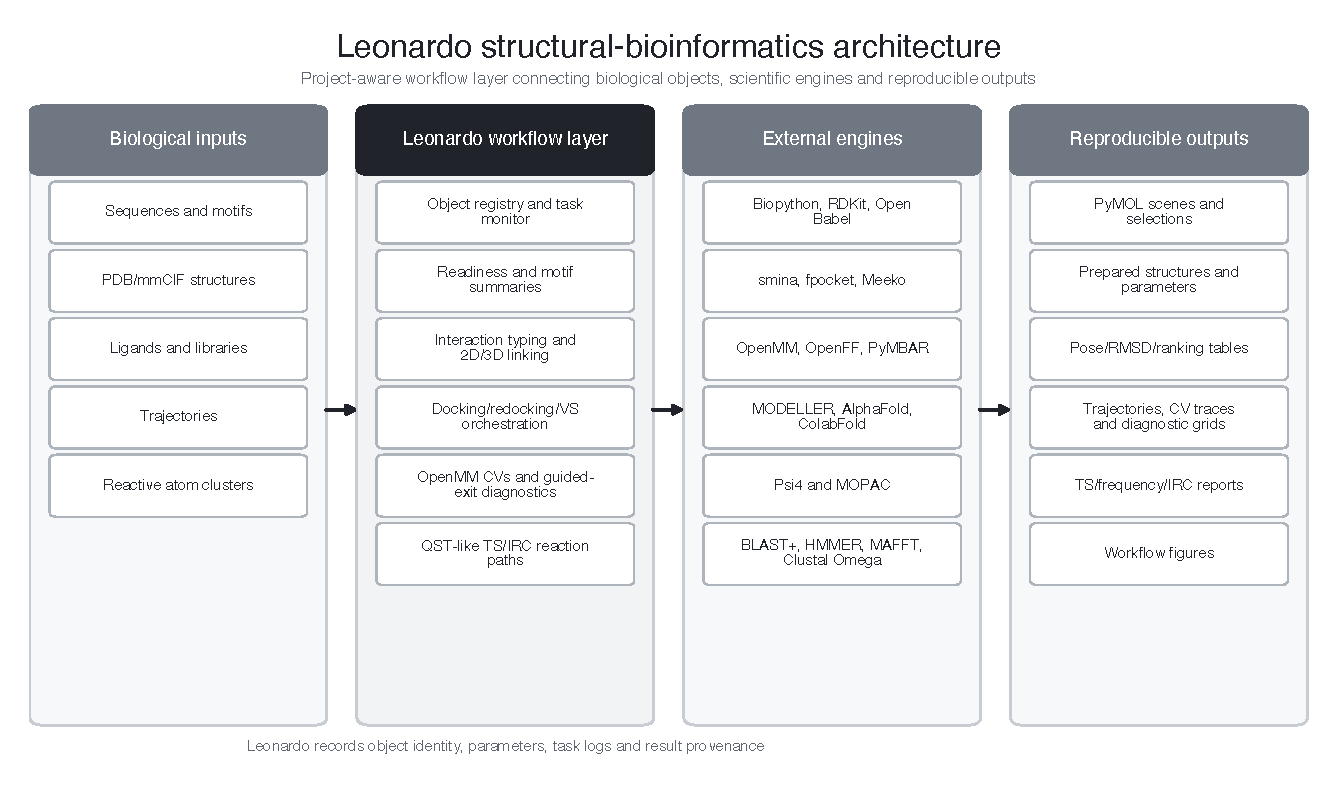
\includegraphics[width=\textwidth]{../figures/figure_1_workflow_architecture.pdf}
\caption{Leonardo workflow architecture.  Biological inputs are managed by Leonardo workflows, which call specialized external engines and return PyMOL scenes, prepared structures, tables, reports and figures.  The contribution boundary is the project-aware GUI, object mapping, workflow verification, reporting and plotting layer; specialized engines provide the cited numerical methods.}
\label{fig:workflow}
\end{figure}

The architecture is exposed to users through a single workflow launcher that keeps structure-loading controls, ligand-state summaries, interaction controls, module entry points and task-monitoring utilities visible in one place (Figure~\ref{fig:suiteinterface}).  This interface is intended to make the suite usable as a coherent structural-bioinformatics workspace rather than as a collection of disconnected scripts.

\begin{figure}[htbp]
\centering
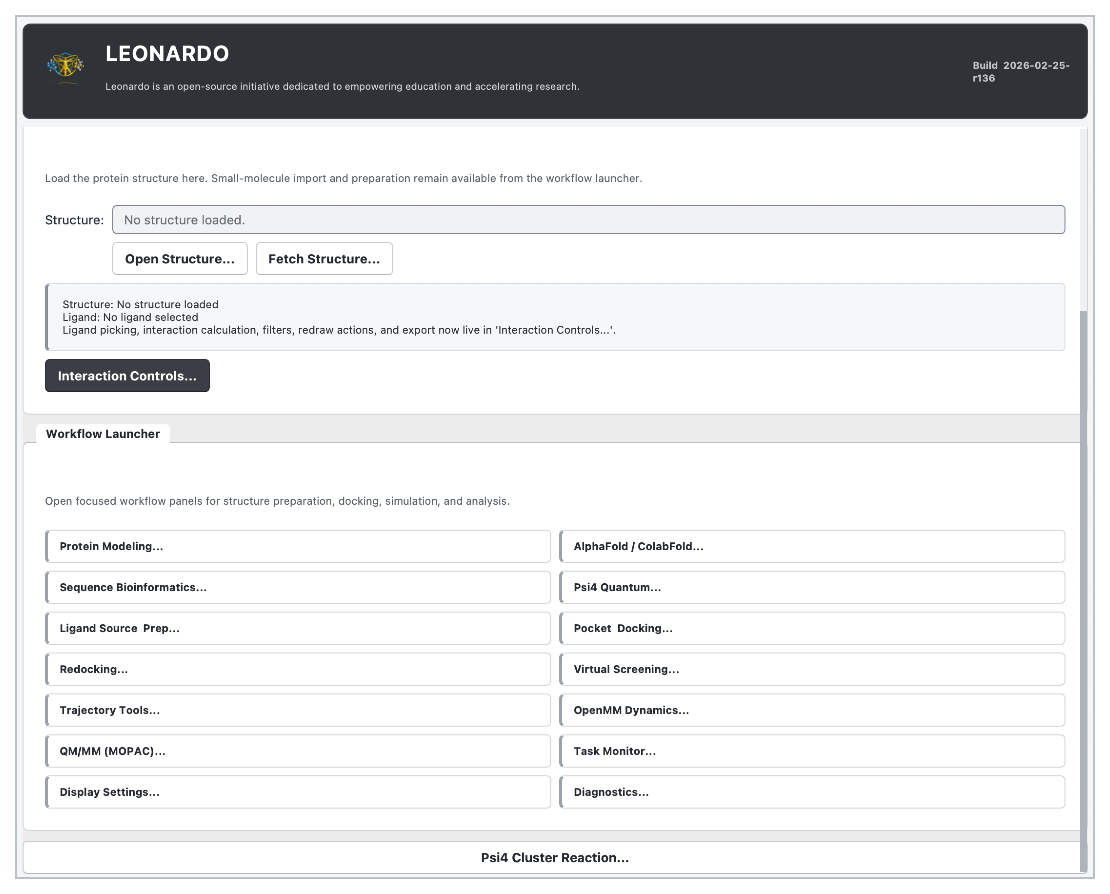
\includegraphics[width=\textwidth]{../figures/figure_0_leonardo_suite_interface.pdf}
\caption{Leonardo suite interface.  The main window provides structure loading and fetching, ligand and interaction-state summaries, interaction controls, workflow-launch buttons for the major modules and access to task monitoring and diagnostics.  The screenshot documents the user-facing integration layer that connects PyMOL objects to Leonardo workflow modules.}
\label{fig:suiteinterface}
\end{figure}

The module comparison identified six pipeline groups: inputs/project state, sequence/structure preparation, protein-ligand modeling, simulation/free-energy analysis, quantum/reaction paths and prediction/external compute.  Across the 15 modules Leonardo orchestrates more than 30 cited external tool or service dependencies, with dependency breadth ranging from two to six tools per module.  Workflow-support categories include automated tests, workflow checks, case demonstrations, report/guardrail checks and rendered figures (Figure~\ref{fig:pipelinestats}).  These categories document implemented software surfaces and available checks; they do not assign equal scientific validation strength to every module.

\begin{figure}[htbp]
\centering
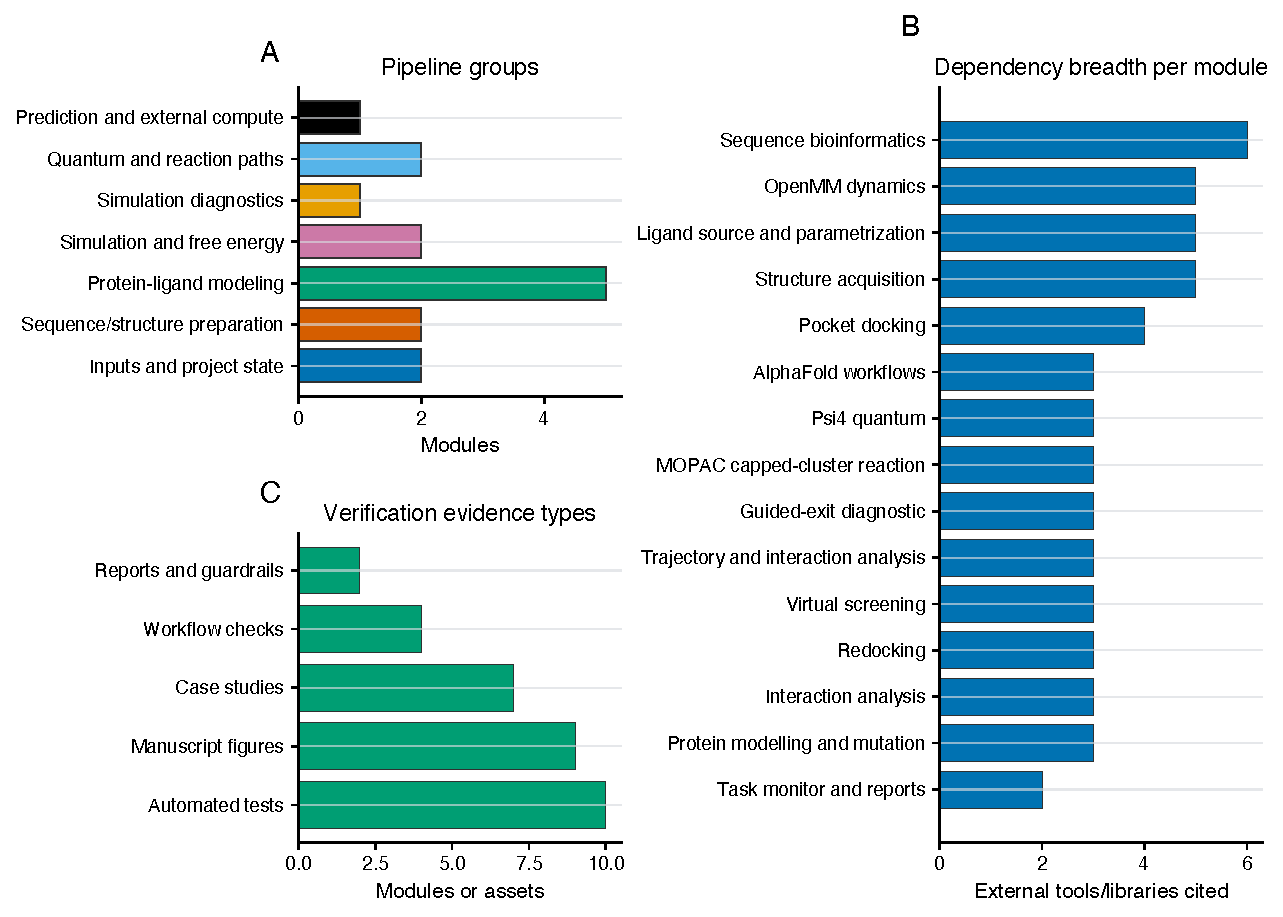
\includegraphics[width=\textwidth]{../figures/figure_2_pipeline_inventory.pdf}
\caption{Module inventory for $n=15$ Leonardo modules.  (A) Module counts by workflow group.  (B) Number of cited external tools or services per module.  (C) Workflow-support categories represented in tests, workflow checks, case demonstrations, reports and rendered outputs.  Counts are manual workflow categories rather than independent scientific performance measurements.}
\label{fig:pipelinestats}
\end{figure}

The module workflow-feature matrix provides a more granular view of these comparisons (Figure~\ref{fig:evidencematrix}).  Adapter modules such as AlphaFold workflows and pocket docking are represented by object handoff, workflow execution or report generation.  Native pipelines such as interaction analysis, redocking, OpenMM dynamics and the Psi4/MOPAC reaction modules show additional support artifacts for plotting, case examples or repeated sampling.  The matrix is an inventory of implemented workflow surfaces and available checks; it is not intended to rank scientific validation strength across modules.

\begin{figure}[htbp]
\centering
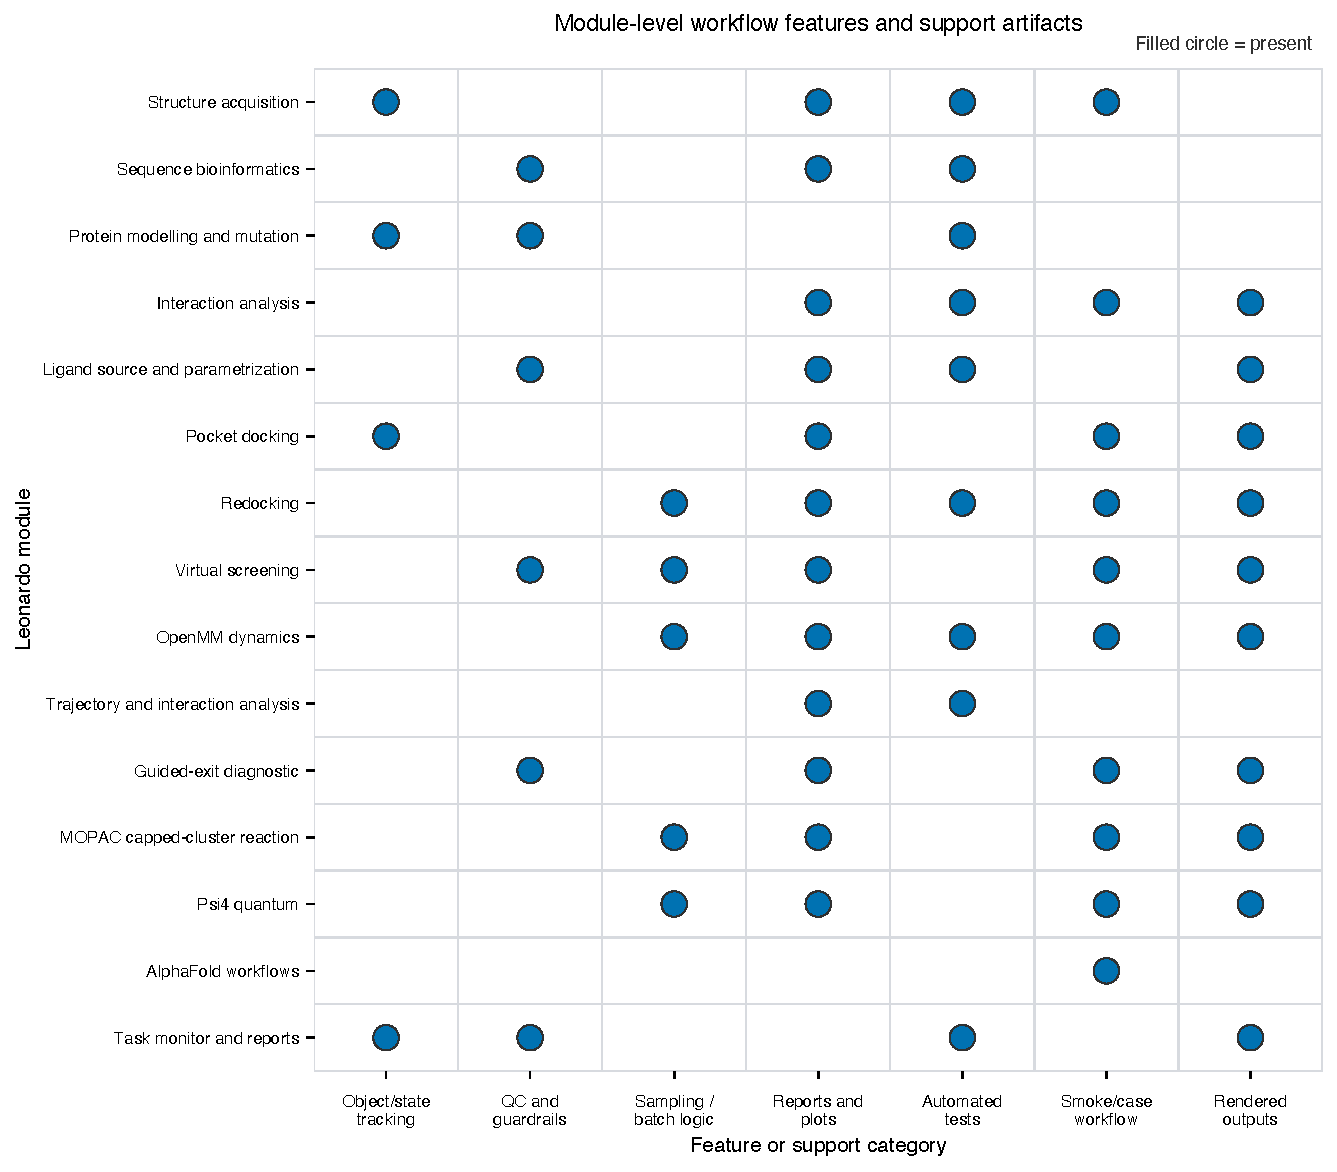
\includegraphics[width=\textwidth]{../figures/figure_3_module_evidence_matrix.pdf}
\caption{Module-level workflow features and support artifacts.  A filled circle indicates that the module contains the corresponding workflow capability, workflow check, case example, automated test or rendered output.  Symbols do not encode scientific benchmark strength or compare accuracy across modules.}
\label{fig:evidencematrix}
\end{figure}
\FloatBarrier

\subsection{Modules that expose established tools}

\subsubsection{Structure acquisition}

The structure-acquisition module is an adapter around public structural resources and PyMOL object creation.  It fetches experimental structures from the Protein Data Bank and imports predicted or local models while preserving source, chain and object names for downstream modules \cite{pdb2000}.  Leonardo does not implement a new structure-prediction or structure-archive algorithm in this module; its purpose is to prevent ambiguous receptor objects and undocumented file handoffs.  A typical use is to load an apo enzyme, a holo PDB structure and a predicted model into the same PyMOL project before selecting the receptor used for docking or mutation analysis.

\subsubsection{AlphaFold and ColabFold workflows}

The AlphaFold module prepares local or Google Colab ColabFold runs by transferring the working sequence, job name and selected parameters into a runnable prediction workflow \cite{alphafold2021,colabfold2022}.  The scientific prediction is performed by AlphaFold/ColabFold, not by Leonardo.  Leonardo contributes sequence export, parameter transfer, result import and model inspection inside the same project.  This is useful when a user has a UniProt sequence but no experimental structure, or when a predicted domain model is needed before ligand-pocket inspection.

\subsubsection{Bioinformatics sequence analysis}

The sequence-analysis module connects sequence records to UniProt motif summaries, readiness reports and alignment/search handoffs to BLAST+, HMMER, MAFFT and Clustal Omega \cite{uniprot2025,blastplus2009,hmmer2011,mafft2013,clustalo2011}.  This module does not replace those algorithms.  Its role is to bring motif positions, residue numbers and sequence context into pop-up summaries that can guide structural work.  For example, a user can identify a catalytic motif, map its residues onto a model and then decide which positions should be included in mutation modeling or interaction analysis.

\subsubsection{Protein modeling and mutation}

Protein modeling and mutation is a guided adapter around MODELLER, Biopython and PyMOL inspection \cite{modeller1993,biopython2009,pymol}.  Leonardo prepares mutation choices, template/model handoff, repair checks and scene updates, while comparative modeling and structural parsing are performed by the external tools.  The module is intended for biological questions such as whether a resistance mutation is near a binding site, whether a missing loop should be modelled before docking, or whether a mutation disrupts a salt bridge seen in the interaction-analysis module.

\subsubsection{Ligand source and parametrization}

The ligand-source and parametrization module manages chemical inputs before docking, simulation or quantum calculations.  It uses RDKit and Open Babel for parsing and conversion, and prepares handoffs to Meeko, AmberTools, OpenFF or quantum-derived charge workflows where appropriate \cite{rdkit,openbabel2011,meeko,ambertools,openff2018}.  Leonardo does not claim a new force-field or protonation algorithm here.  Its value is ligand registry management, format checks, charge/protonation warnings and consistent downstream object selection.  In practice, this module helps detect failed SDF records, suspicious formal charges or inconsistent ligand identifiers before a screening or MD job is launched.

\subsubsection{Pocket docking}

Pocket docking is an adapter workflow around pocket detection, docking-grid definition and docking execution with tools such as fpocket, Meeko and smina \cite{fpocket2009,smina2013,meeko}.  The scoring and pose search are performed by the docking engine.  Leonardo contributes object-aware receptor/ligand selection, pocket-to-grid handoff and pose visualization so the user knows exactly which protein and ligand objects were used.  The workflow check reported here evaluates object handoff and report generation for the pocket-docking workflow; it does not assess pocket-detection accuracy, docking pose accuracy or scoring performance.  A typical use is to compare a crystallographic pocket with an automatically detected pocket before docking a focused inhibitor series.

The pocket-docking workflow example parsed fpocket output with 10 detected pockets, selected pocket 4 by the configured ranking criterion, constructed a docking grid centered at $(8.94, 6.52, 8.50)$ \AA{} with dimensions $(11.43, 16.36, 11.56)$ \AA{} and parsed three smina pose modes for the selected pocket.  To address crystallographic-site recovery separately from the smoke workflow, fpocket was also run on the 1STP receptor after removing biotin.  The recovered pocket with the smallest ligand-to-alpha-sphere distance was pocket 1; all 16 biotin heavy atoms were within 4 \AA{} of an alpha sphere and the median atom-to-alpha-sphere distance was 0.90 \AA{}.  Figure~\ref{fig:pocketdocking} summarizes the pocket ranking, pocket physicochemical descriptors, selected-pocket/grid geometry and docking-mode affinity/RMSD information, while the 1STP/biotin pocket-overlap values are provided in \texttt{draft/results/pocket\_1stp\_crystal\_overlap.csv}.  These checks support Leonardo's pocket-to-grid and pose-summary reporting path; they are not a broad benchmark of pocket detection or docking scoring.

\begin{figure}[htbp]
\centering
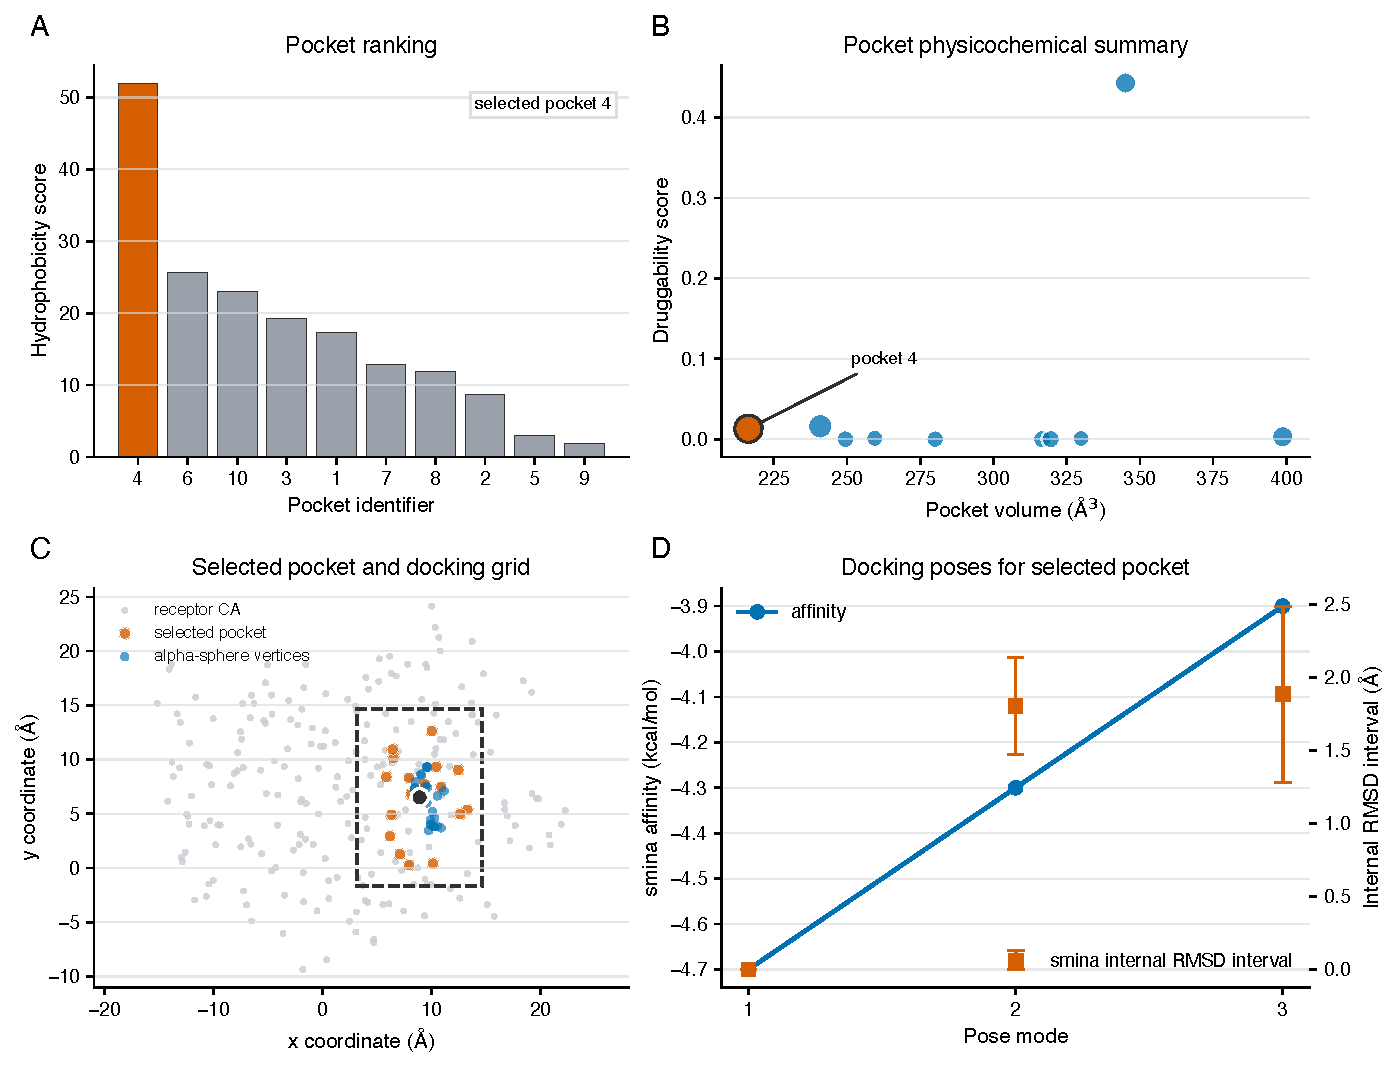
\includegraphics[width=\textwidth]{../figures/figure_11_pocket_docking_workflow_check.pdf}
\caption{Pocket-docking workflow check using fpocket and smina outputs.  The example parsed $n=10$ fpocket pockets, selected pocket 4 using the configured ranking rule and constructed the docking grid from that selected pocket.  (A) Pocket ranking by hydrophobicity score with the selected pocket highlighted.  (B) Pocket volume versus druggability score, with marker size proportional to the number of alpha spheres.  (C) Two-dimensional projection of the receptor, selected pocket alpha-sphere/atom records and generated docking grid.  (D) smina affinity and the internal lower/upper-bound RMSD interval reported by smina for the parsed pose modes; this is not a crystal-template RMSD.  A separate 1STP/biotin crystal-site overlap check recovered fpocket pocket 1 with 100\% of biotin heavy atoms within 4 \AA{} of an alpha sphere.  The figure checks handoff and reporting, not pocket-detection or docking accuracy.}
\label{fig:pocketdocking}
\end{figure}

\subsubsection{Task monitor and reports}

The task monitor is a support module rather than a scientific algorithm.  It records background jobs, opens logs, summarizes failures and keeps workflow metadata accessible.  Its purpose is practical reproducibility: a failed smina, OpenMM, Psi4, MOPAC or ColabFold run should produce a readable error summary rather than a silent GUI failure.  This module is useful in teaching and shared-lab settings where users need to know which step failed and which input object or executable caused the problem.

\subsection{Scientific workflow pipelines implemented in Leonardo}

\subsubsection{Protein-ligand interaction analysis}

The interaction-analysis module is a Leonardo workflow pipeline because contact classification, residue grouping, charge guardrails and 2D-to-3D selection are implemented in Leonardo.  The pipeline reduces atom-level observations to residue-level records.  For ligand atoms $L$ and receptor-residue atoms $R_r$, the closest residue-ligand distance is
\begin{equation}
d_{\min}(r,L)=\min_{i \in R_r,\; j \in L} \left\| \mathbf{x}_i-\mathbf{x}_j \right\|_2 .
\end{equation}
Candidate contacts are retained only when distance, element type, residue context and interaction-specific geometry agree.  Salt bridges require opposite formal-charge evidence and charged-center proximity; nitrogen atoms are not treated as cations solely because they are nitrogen.  This conservative rule is important because bad ligand protonation, missing hydrogens or wrong formal charges would otherwise create false electrostatic interactions.

The 3PTB benzamidine case contained 1629 protein atoms across 223 residues and nine ligand heavy atoms.  The reproducible contact analysis used Leonardo's shared runtime criteria for charge-group, hydrogen-bond fallback, hydrophobic and van der Waals checks, then reduced atom-level contacts to residue-level records.  The resulting table contained 15 residue-level contacts: one side-chain hydrophobic contact, four polar contacts, one salt-bridge candidate and nine non-directional close contacts.  This case checks parsing, residue-level grouping, conservative contact labeling for the interaction classes observed in 3PTB/BEN and plot generation.  It does not constitute a benchmark against curated interaction annotations, and interaction classes absent from this structure require separate future comparison against external tools or curated complexes.  The implemented framework also contains rules for hydrogen bonds, halogen bonds, aromatic interactions, cation-pi contacts, metal contacts and hydrophobic/van der Waals clusters, following principles used in protein-ligand interaction profilers \cite{plip2015}; those classes are reported here as implemented capability, not as fully benchmarked chemistry.  The module is used to ask whether a ligand analog preserves key binding contacts, whether a mutation removes a salt bridge or whether a docking pose reproduces interactions seen in a reference structure.

\begin{figure}[htbp]
\centering
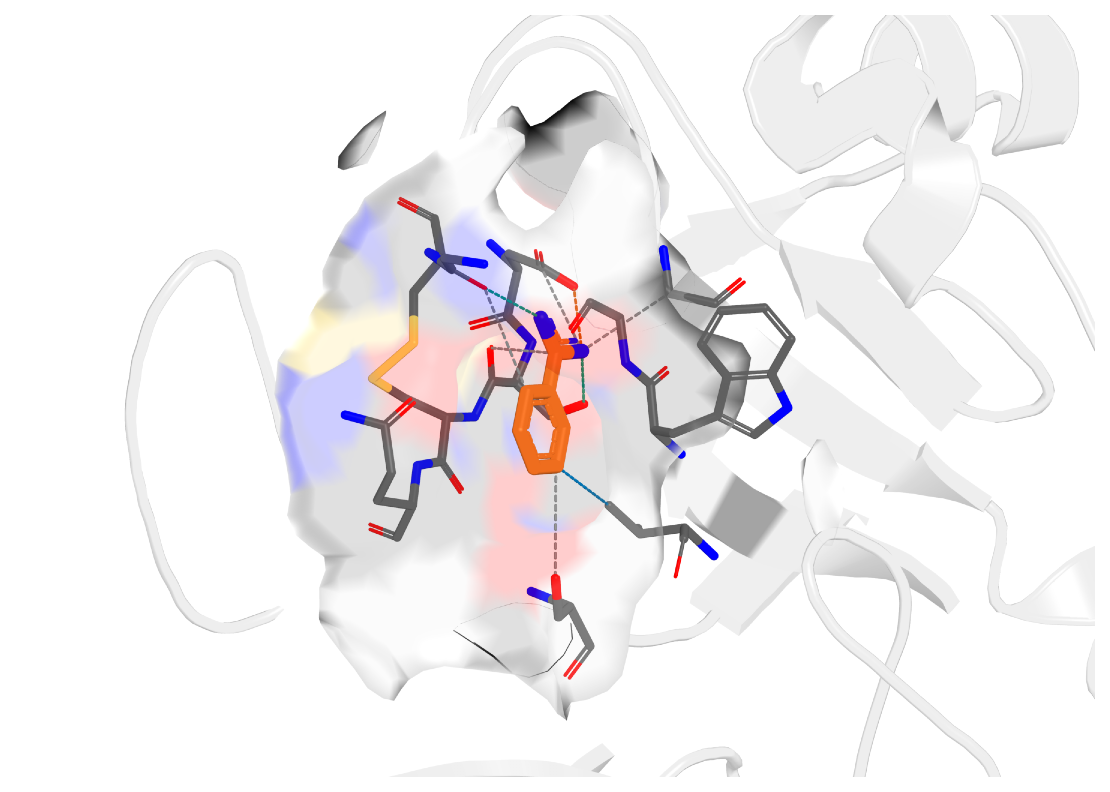
\includegraphics[width=\textwidth]{../figures/figure_4b_3ptb_ben_interaction_scene.pdf}
\caption{Protein-ligand interaction scene generated by Leonardo for the 3PTB/benzamidine case.  The PyMOL-rendered image shows the ligand in the trypsin binding site, retained contact residues as sticks, a semi-transparent pocket surface and color-coded dashed contact-distance objects derived from Leonardo's contact table.  Dashed contacts use the same class colors as Figure~\ref{fig:interactions}: polar contacts in green, the salt-bridge candidate in orange, hydrophobic contacts in blue and non-directional close contacts in gray.  The scene is intended as a visual interaction report for inspection and communication; quantitative contact counts and distances are summarized separately in Figure~\ref{fig:interactions}.}
\label{fig:interactionscene}
\end{figure}

\begin{figure}[htbp]
\centering
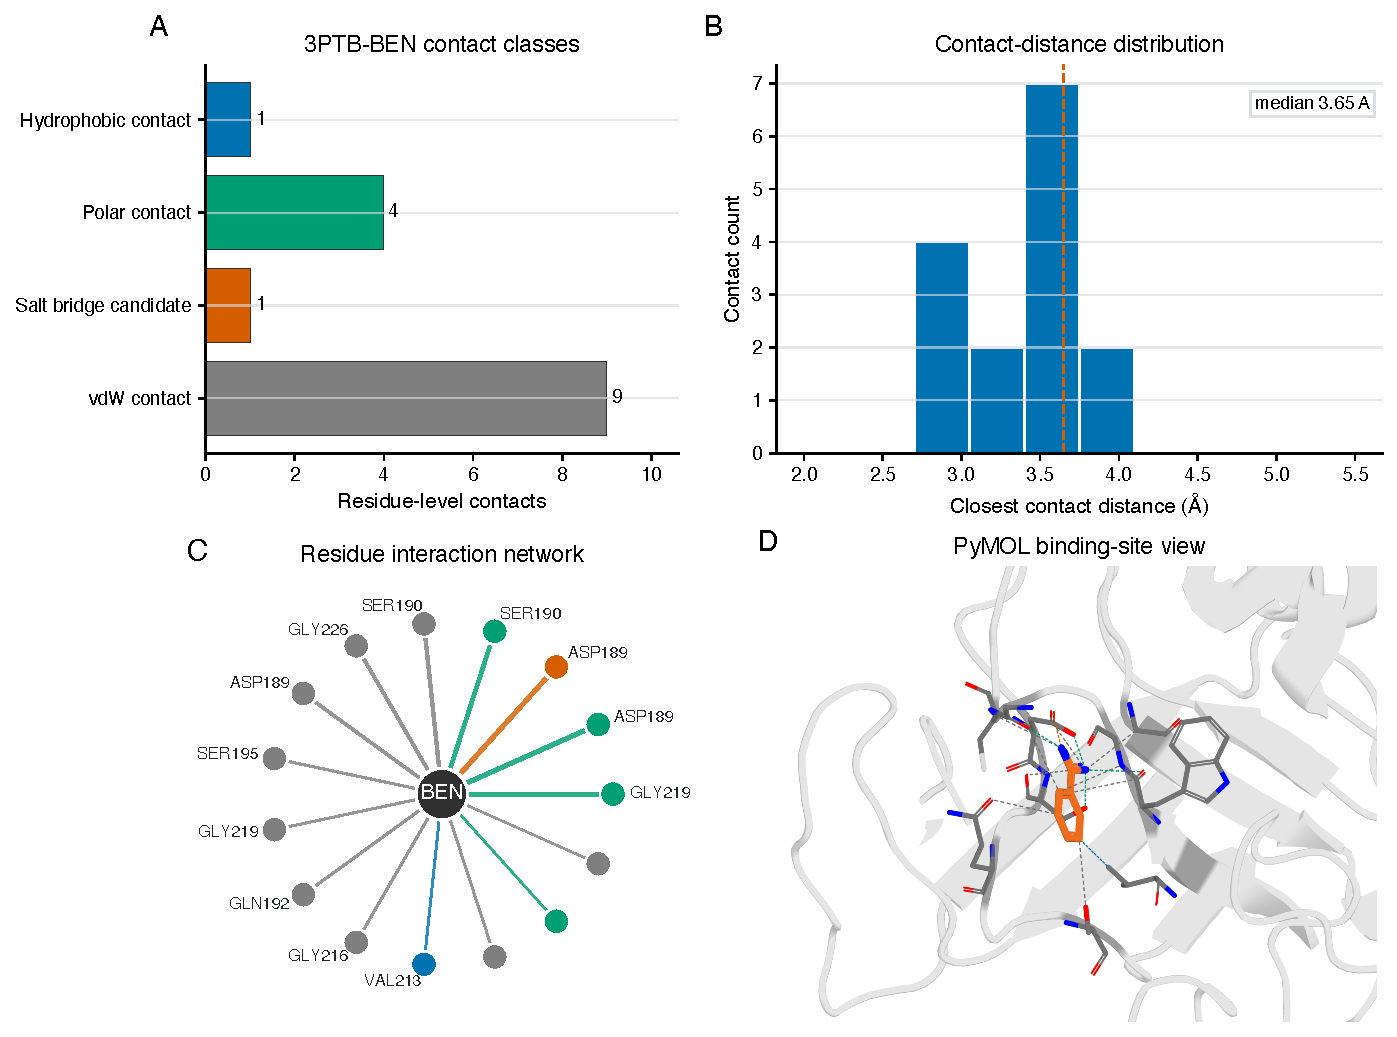
\includegraphics[width=\textwidth]{../figures/figure_4_3ptb_ben_interactions.pdf}
\caption{3PTB benzamidine contact case demonstration.  The case contains $n=15$ retained residue-level contacts from PDB 3PTB and ligand BEN using the workflow input charge/protonation state and conservative charge-aware typing.  (A) Residue-level contact counts by conservative class.  (B) Closest-distance distribution for retained contacts.  (C) Residue-level interaction network linking BEN to retained contact residues; repeated residue labels indicate multiple retained atom-level contacts collapsed to residue-level summaries.  (D) PyMOL-rendered binding-site view showing BEN, retained contact residues and dashed contact-distance objects generated from the same contact table.  The figure summarizes observed retained contacts and is not a curated benchmark of absent interaction classes.}
\label{fig:interactions}
\end{figure}

\subsubsection{Redocking}

The redocking module is a Leonardo workflow pipeline around smina docking.  The docking search and affinity scoring are performed by smina, while Leonardo carries a crystallographic template ligand through preparation, runs repeated seeds, parses all modes and reports both docking score and template recovery.  For the manuscript script, receptor and template coordinates are prepared in a common crystal frame before docking, and template recovery is reported as no-fit heavy-atom RMSD using the order-preserving heavy-atom correspondence generated from the same Open Babel ligand template:
\begin{equation}
\mathrm{RMSD}_\mathrm{nofit}=\sqrt{\frac{1}{N}\sum_{i=1}^{N}\left\| \mathbf{x}_i-\mathbf{y}_{\pi(i)} \right\|^2 } ,
\end{equation}
where $\pi$ is the retained atom correspondence for this prepared template/pose pair.  The reported value is therefore appropriate for the 1STP/biotin workflow check but is not presented as a symmetry-corrected ligand-RMSD benchmark for arbitrary chemotypes.  In workflows that require receptor alignment before redocking, Leonardo stores the alignment transform separately as a preparation quality-control step; the final ligand recovery value is only reported when an explicit reference ligand is available.

In a single 1STP/biotin redocking case using an explicit crystallographic template and known binding-site grid, 15 seed runs produced 225 pose rows.  Each seed generated 15 smina modes, and every seed recovered at least one pose below the common 2.0 \AA{} heavy-atom RMSD success threshold.  Across the 15-seed run, the top-scored pose median RMSD was 0.363 \AA, the best-pose median RMSD was 0.358 \AA, and the minimum observed RMSD was 0.331 \AA.  These seeds probe workflow reproducibility and stochastic docking variation for one target; they are not independent target-level benchmark replicates.  This demonstrates receptor/ligand preparation, seed repetition, preserved-correspondence RMSD reporting and smina-output parsing for this case; it does not test smina scoring accuracy, flexible-receptor treatment or redocking performance across targets.  The plot also shows why Leonardo displays both docking score and RMSD-derived recovery metrics when a template ligand is available.

\begin{figure}[htbp]
\centering
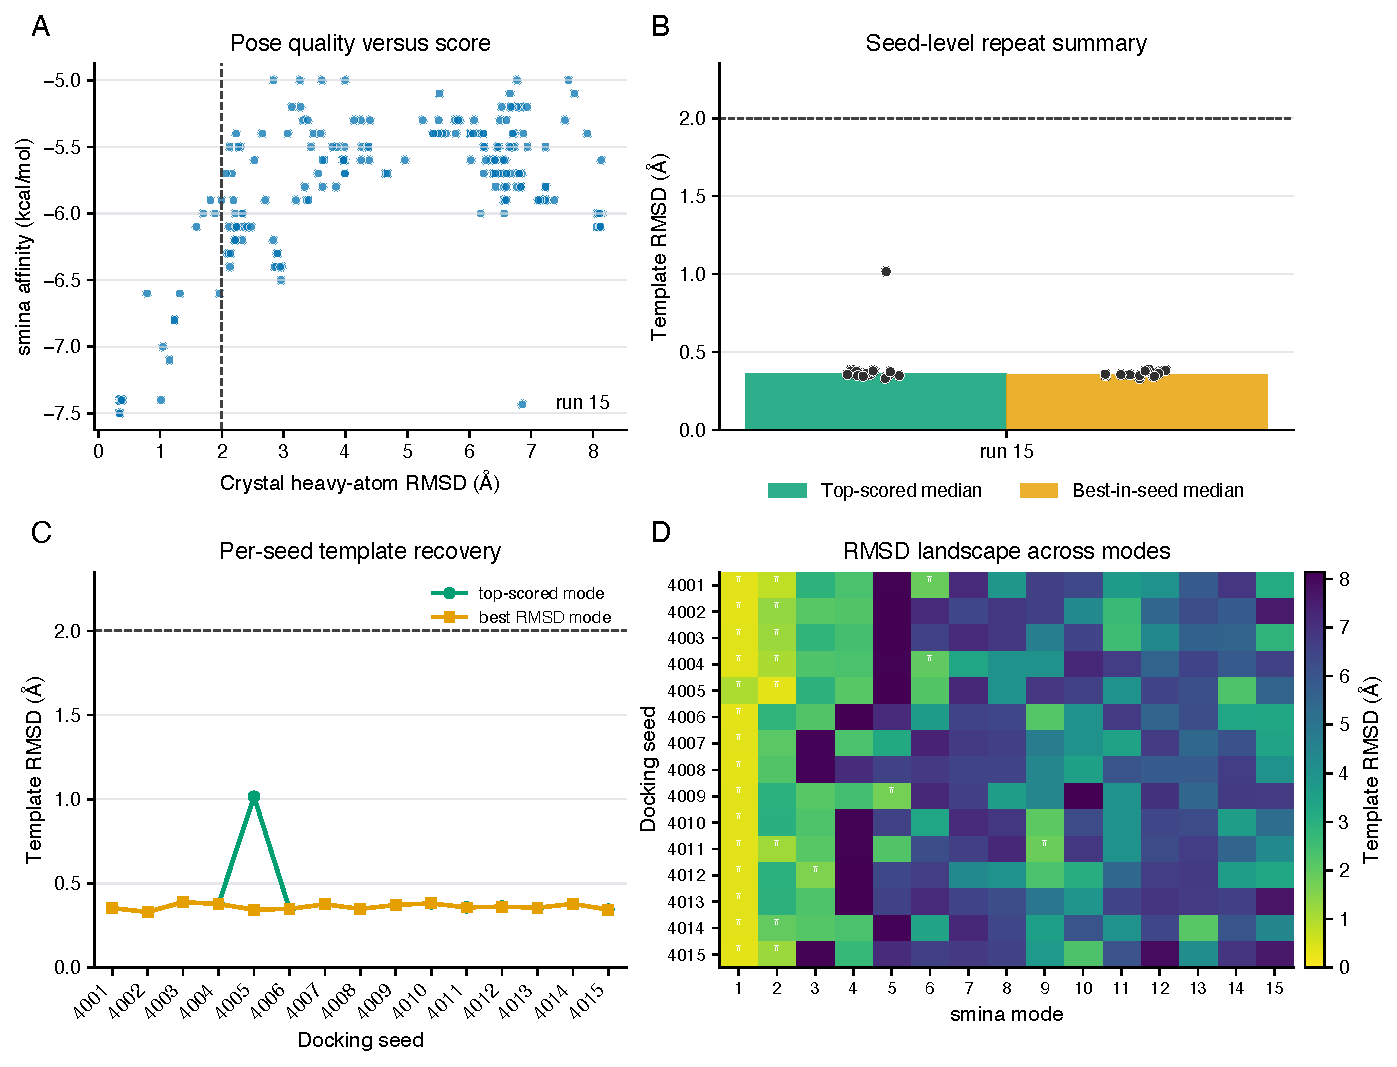
\includegraphics[width=\textwidth]{../figures/figure_5_redocking_1stp_btn.pdf}
\caption{Single-target 1STP biotin template-redocking workflow check.  The case contains $n=225$ pose rows from $n=15$ seed runs, with 15 smina modes per seed.  (A) Template heavy-atom RMSD versus smina affinity for all modes; the dashed line marks 2.0 \AA.  (B) Median top-scored and best-per-seed template RMSD with individual seed-level points overlaid.  (C) Per-seed template recovery for top-scored and best-RMSD modes.  (D) RMSD landscape across smina modes and seeds; asterisks mark modes below 2.0 \AA.  This checks Leonardo's template mapping and reporting for this case, not general docking accuracy.}
\label{fig:redocking}
\end{figure}

\subsubsection{Virtual screening}

The virtual-screening module is a Leonardo batch-docking and ligand-library workflow around RDKit, Meeko and smina.  Leonardo does not introduce a new scoring function; the default rank is the ordered docking affinity returned by the docking engine,
\begin{equation}
\mathrm{rank}(i)=\mathrm{order}\left(E_i^\mathrm{dock}\right),
\end{equation}
with lower predicted binding energy ranked first.  Leonardo adds the pieces that make the run reproducible for non-specialist users: ligand-library parsing, receptor/ligand object selection, batch job creation, failure reporting, hit-table generation and PyMOL handoff of selected poses.

The ligand-library quality-control demonstration used RDKit to parse 369 molecules across 15 curated local SDF files named by target.  In addition to molecular descriptors, the workflow records parsed versus failed SDF records, formal-charge flags, multi-fragment records, unassigned stereocenters and duplicate canonical SMILES counts before downstream docking preparation.  The median molecular weight was 388.5 Da and the median calculated logP was 3.39.  The target-level ligand counts, molecular-property panel and machine-readable QC table provide a quality-control layer before virtual screening, helping users detect empty libraries, failed SDF parsing, charge/stereo issues or chemical-space mismatches before launching docking jobs.  This is not a virtual-screening enrichment benchmark: no actives/decoys, ROC-AUC, enrichment factor, BEDROC, retrospective ranking or prospective hit validation is reported here, and such metrics require appropriate benchmark design \cite{truchon_vsmetrics2007}.  In practical use, this module supports triage of focused inhibitor libraries, comparison of analog series and selection of candidate poses for interaction analysis or follow-up MD.

\begin{figure}[htbp]
\centering
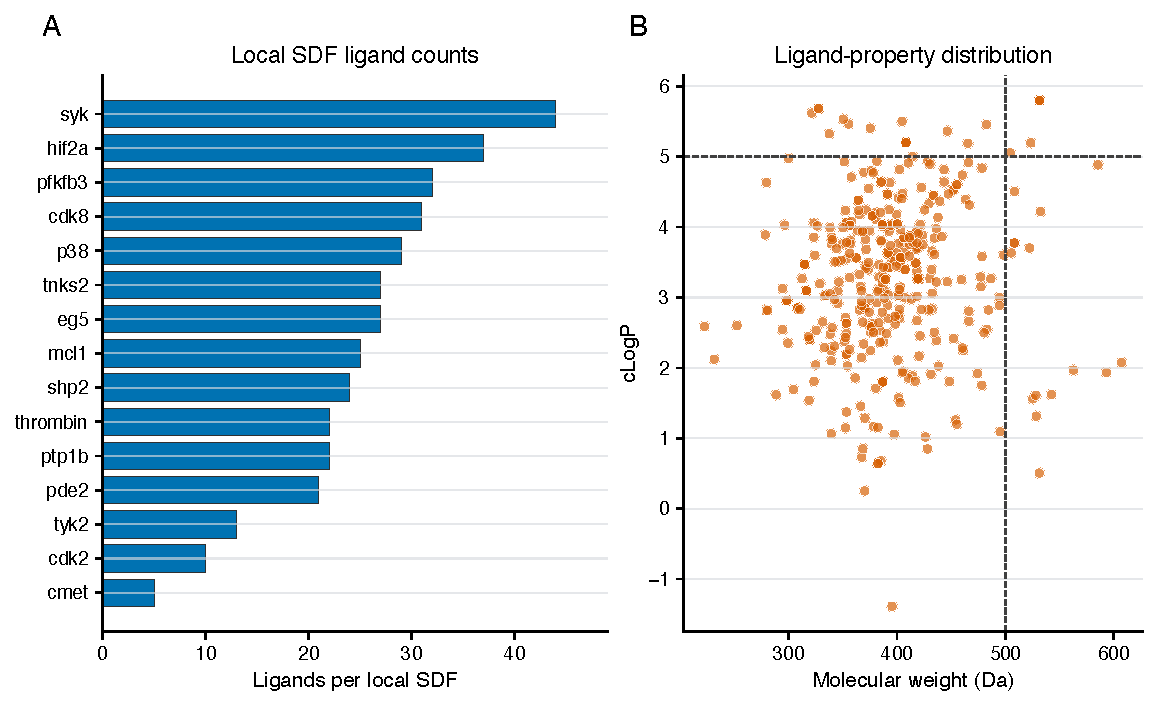
\includegraphics[width=\textwidth]{../figures/figure_6_ligand_library_qc.pdf}
\caption{Local ligand-library quality-control demonstration.  RDKit parsed $n=369$ molecules across 15 local SDF target files.  (A) Ligand counts per target.  (B) Molecular weight and calculated logP distribution; dashed lines at 500 Da and logP 5 are heuristic QC references, not pass/fail criteria or virtual-screening enrichment evidence.}
\label{fig:ligands}
\end{figure}

\subsubsection{OpenMM dynamics, collective variables and diagnostic grids}

The OpenMM dynamics module is a Leonardo setup and analysis pipeline around OpenMM, OpenFF, AmberTools, PyMBAR and MDTraj \cite{openmm2017,openff2018,ambertools,mbar2008,mdtraj2015}.  Leonardo prepares protocol stages, exposes predefined collective variables and plots collective-variable traces and diagnostic metadynamics-grid outputs.  The module can prepare umbrella or metadynamics-style workflows using established enhanced-sampling concepts \cite{torrie_umbrella1977,kumar_wham1992,laio_metadynamics2002}; the manuscript example exercises setup and plotting rather than comparing enhanced-sampling algorithms.  In the alanine example, Leonardo reads OpenMM metadynamics grid values and displays a shifted diagnostic surface,
\begin{equation}
G_\mathrm{plot}(\phi,\psi)=G_\mathrm{OpenMM}(\phi,\psi)-\min_{\phi,\psi}G_\mathrm{OpenMM}(\phi,\psi),
\end{equation}
with clipping used only for visualization.  This display is not an unbiased histogram PMF, WHAM/MBAR estimate or uncertainty-calibrated thermodynamic free-energy surface.

The OpenMM workflow example used ACE-ALA-NME to exercise Leonardo's collective-variable and diagnostic-grid plotting machinery on a compact CPU-compatible system.  The phi/psi run produced 2304 grid rows and passed Leonardo's internal plotting-stability criterion after 43,000 steps: the RMSD between consecutive shifted grids remained below 0.5 kJ mol$^{-1}$ for five consecutive blocks.  This is a backend and plotting criterion, not a claim of physically converged alanine thermodynamics.  A companion CV trace panel exercised eight Leonardo CV presets on the same alanine-dipeptide model, with representative distance, RMSD, torsion and angle traces normalized to z-scores for plotting.  This example demonstrates setup, metadynamics-style execution, plotting-stability tracking and figure generation on a small molecule; it is not intended as a biological protein-scale free-energy benchmark or an uncertainty-calibrated force-field study.  In real workflows this module is used to prepare minimization/heating/equilibration protocols, explore torsional sampling, test umbrella or metadynamics CVs and inspect sampling stability before running larger protein systems.

\begin{figure}[htbp]
\centering
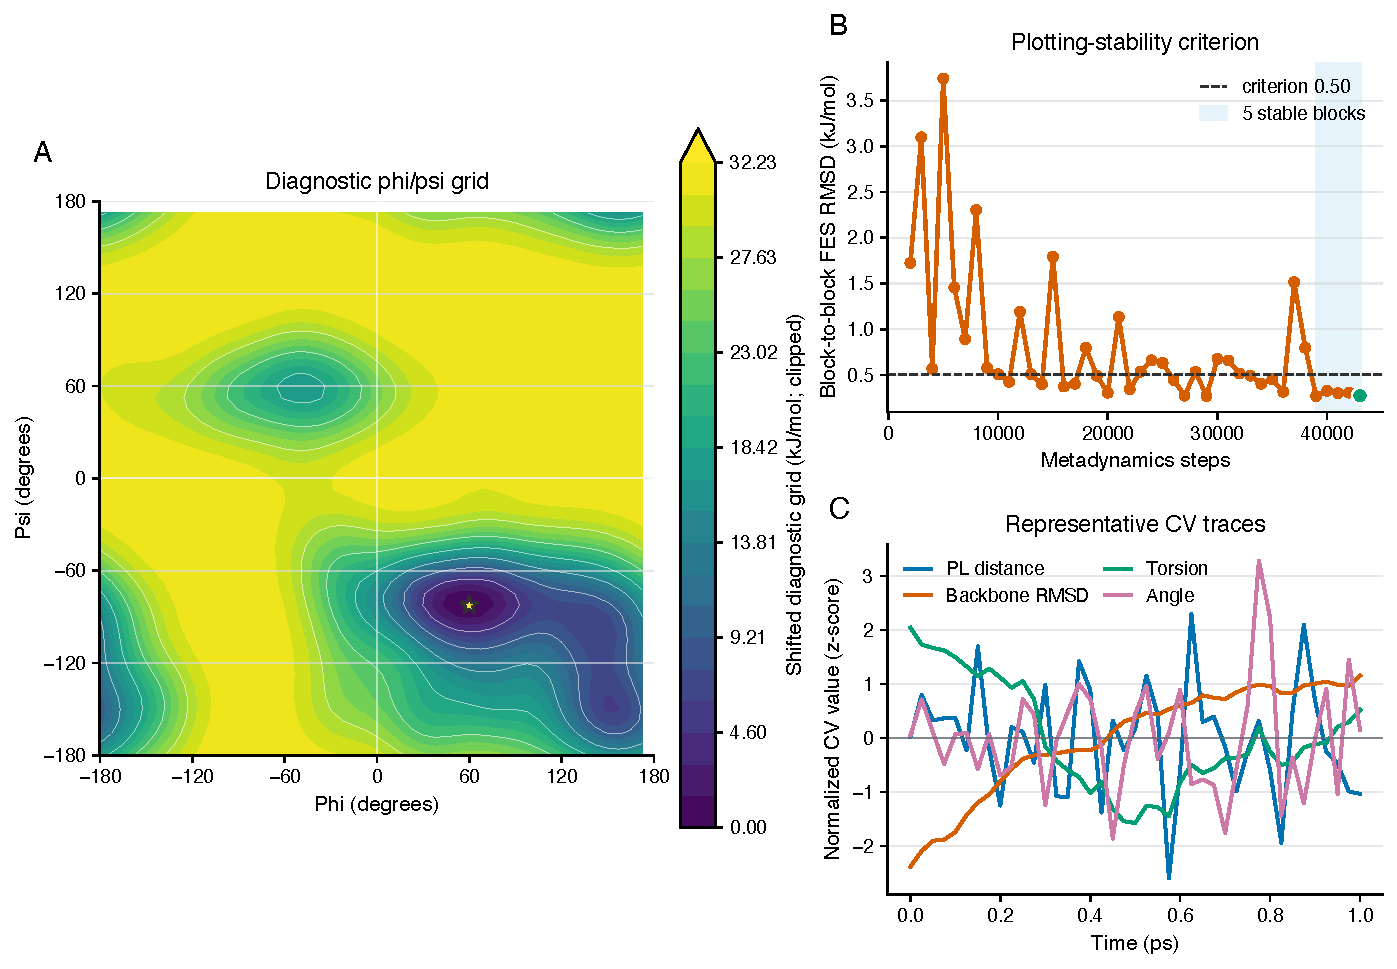
\includegraphics[width=\textwidth]{../figures/figure_7_openmm_cv_fes_workflow_check.pdf}
\caption{OpenMM/CV backend check on ACE-ALA-NME.  The phi/psi metadynamics-style run used 2304 diagnostic grid rows and passed Leonardo's internal plotting-stability criterion after 43,000 steps.  (A) Shifted metadynamics diagnostic grid with the global minimum marked; the displayed color scale is clipped at the 97.5th percentile only for visualization.  (B) Block-to-block shifted-grid RMSD trace; the shaded region marks the final five consecutive blocks below the 0.5 kJ mol$^{-1}$ threshold.  (C) Representative CV traces normalized to z-scores so different CV units are not mixed on one physical scale.  The panel checks Leonardo's setup, plotting-stability tracking and plotting workflow on a compact molecule, not a biological protein-scale free-energy benchmark.}
\label{fig:openmm}
\end{figure}

\subsubsection{Trajectory and interaction analysis}

The trajectory-analysis module is a Leonardo analysis pipeline for MD output.  It uses MDTraj/NumPy for trajectory parsing and numerical operations, but Leonardo defines the contact-occupancy summaries, report structure and PyMOL-linked interpretation.  For a residue-ligand contact $c$ over $T$ trajectory frames, contact occupancy is computed as
\begin{equation}
O_c=\frac{1}{T}\sum_{t=1}^{T}\mathbf{1}\left[d_c(t)<d_\mathrm{cut}\right],
\end{equation}
where $d_c(t)$ is the contact distance at frame $t$, $d_\mathrm{cut}$ is the selected interaction cutoff and $\mathbf{1}$ is an indicator function.  The same framework is used for distance traces, RMSD summaries and persistence reports.  This module is used after MD to decide whether a docking interaction remains stable, whether a residue contact is intermittent or whether a ligand drifted away from the binding site.

\subsubsection{Guided-exit binding diagnostic (historical ABFE-lite module)}

ABFE-lite is the historical module name for Leonardo's resource-constrained guided-exit binding diagnostic workflow for local CPU studies.  In this manuscript the module is reported as a guided-exit diagnostic, not as a production absolute binding free-energy method or a replacement for production alchemical ABFE campaigns, which require carefully designed thermodynamic cycles, restraints, standard-state corrections, uncertainty estimates and repeated sampling \cite{boresch_abfe2003,mey_alchemical2020}.  The workflow constrains resource use, stages analysis and provides restraint diagnostics for preliminary local studies.  The guided-exit option defines a cylinder from a binding-site point to an exit guide point.  If $\mathbf{u}$ is the normalized cylinder axis and $\mathbf{r}$ is the ligand center-of-mass displacement from the binding-site reference, axial progress and radial displacement are
\begin{equation}
z=\mathbf{r}\cdot\mathbf{u}, \qquad \rho=\left\|\mathbf{r}-z\mathbf{u}\right\| .
\end{equation}
The restraint penalizes ligand motion outside the desired exit channel,
\begin{equation}
U_\mathrm{guide}(\rho)=\frac{1}{2}k_\rho \max(0,\rho-\rho_0)^2 ,
\end{equation}
so the ligand is encouraged to leave through the same entrance/exit path instead of escaping through arbitrary protein surfaces.  The current manuscript treats the resulting windows as diagnostic state gates.  Any state-ratio or volume-correction diagnostics emitted by the software are audit outputs from this guided-exit protocol, not production absolute binding free energies.

Here, the guided-exit diagnostic is evaluated as a setup, restraint-design and plotting workflow using the 3PTB/benzamidine system.  A 5 ns guided-exit run generated 2500 sampled records at 2 ps spacing.  The ligand center-of-mass exit coordinate reached 37.84 \AA{}, the maximum-exit frame had a nearest protein-ligand distance of 29.00 \AA{} and no close protein-ligand contacts within 4 \AA{}, and the post-sampling gate accepted 340 bound hold-window records and 69 unbound hold-window records.  These values check that Leonardo can generate, classify, analyze and plot a bound/unbound guided-exit trajectory.  The manuscript diagnostic artifacts retain state-gating and trajectory fields only; no binding affinity, dissociation constant, association constant or IC50 is reported for this diagnostic case.  The result is reported for workflow verification, not as a production ABFE benchmark, ligand-ranking result or binding-affinity estimate.

\begin{figure}[htbp]
\centering
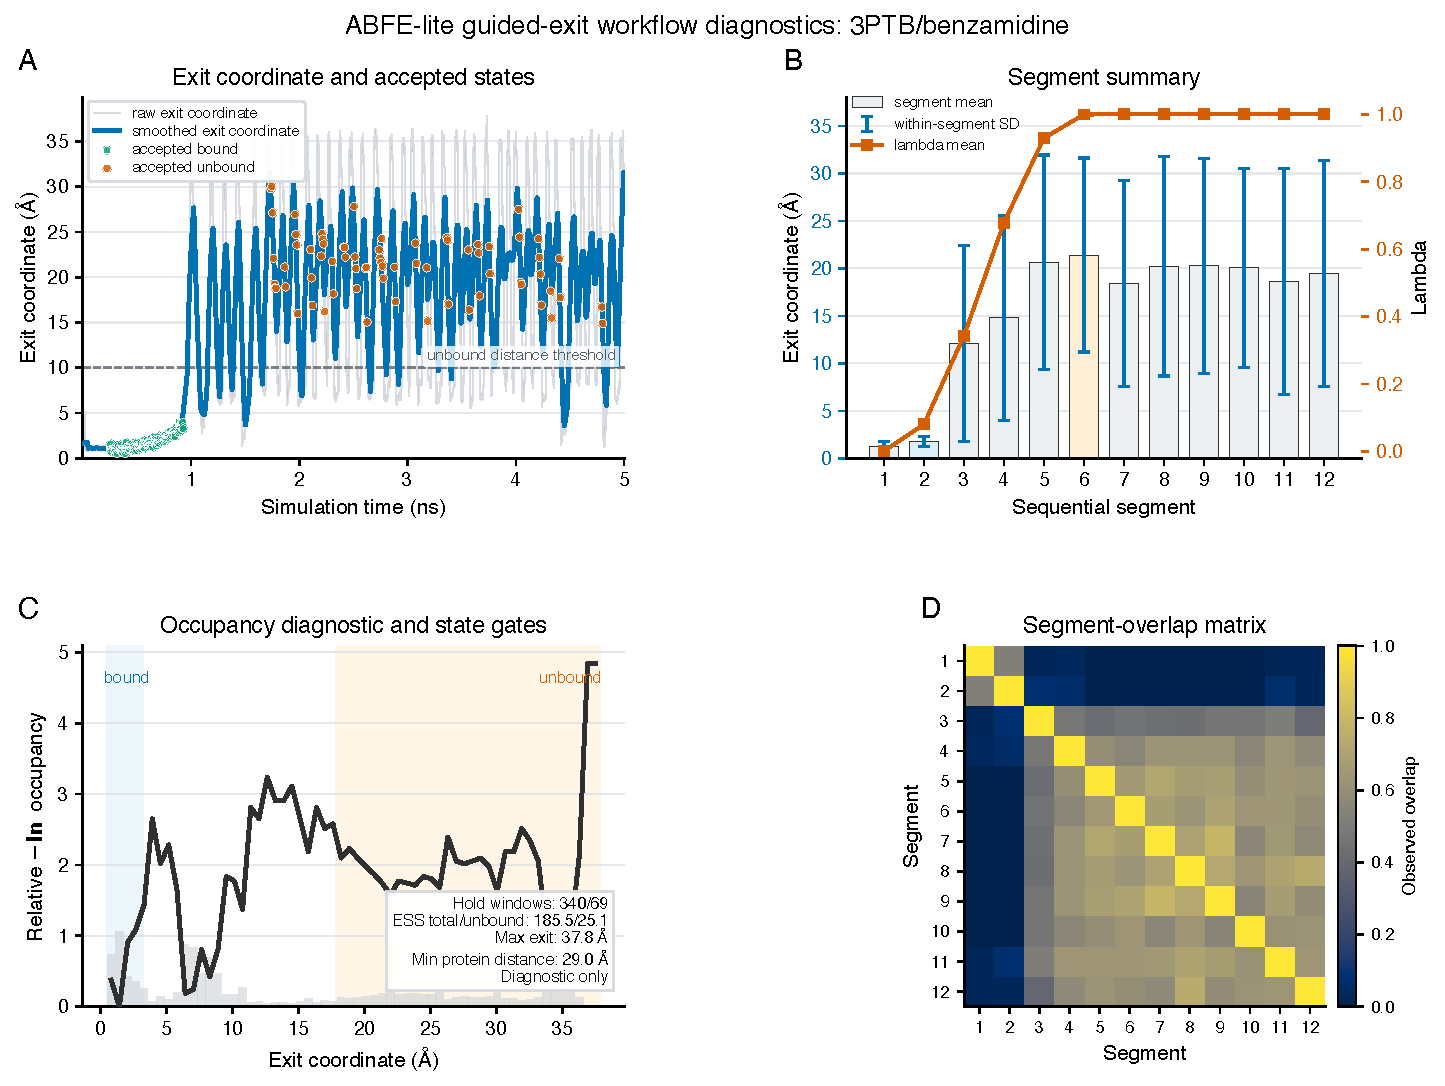
\includegraphics[width=\textwidth]{../figures/figure_10_abfe_lite_diagnostics.pdf}
\caption{Guided-exit binding diagnostic for the 3PTB/benzamidine system.  The historical ABFE-lite module produced 2500 sampled records at 2 ps spacing, divided into 12 sequential analysis segments for plotting.  (A) Real trajectory trace of the binding-site center-of-mass exit coordinate with the steering lambda schedule and state labels; a centered moving average is shown only to declutter the plotted trace.  (B) Segment-level exit-coordinate means, standard deviations and lambda means.  (C) Dimensionless occupancy diagnostic from the sampled trajectory; the accepted diagnostic hold-window counts were 340/69 for bound/unbound states and ESS denotes effective sample size used only as a state-gating diagnostic.  (D) Observed segment-overlap matrix from the real sampled exit-coordinate distributions.  The panel reports a guided-exit workflow check rather than a production absolute binding-free-energy benchmark or binding-affinity estimate.}
\label{fig:abfelite}
\end{figure}

\subsubsection{Psi4 quantum reaction pipeline}

Leonardo includes Python-side reaction-path workflows for Psi4 and MOPAC.  For Psi4, Leonardo generated QST2-like and QST3-like transition-state starting geometries for H + H$_2 \rightarrow$ H$_2$ + H, then delegated transition-state refinement, frequency analysis and IRC execution to Psi4.  The QST2-like and QST3-like transition-state energies differed by only 0.000212 kcal/mol in this compact workflow case.  The frequency analysis reported one imaginary mode with a primary imaginary frequency of 2982.405 cm$^{-1}$, and the resulting IRC profile had a 23.166 kcal/mol relative energy span.

For reaction-path workflows, Leonardo's QST2-like guess construction starts from mapped reactant and product geometries and constructs synchronous-transit guesses along
\begin{equation}
\mathbf{X}(\lambda)=(1-\lambda)\mathbf{X}_\mathrm{R}+\lambda\mathbf{X}_\mathrm{P}, \quad 0 \leq \lambda \leq 1 .
\end{equation}
The QST3-like variant incorporates an additional transition-state estimate $\mathbf{X}_\mathrm{TS}^{(0)}$ to bias the search near a chemically informed saddle region.  A transition-state candidate is accepted only if frequency analysis identifies one dominant imaginary mode.  The IRC driver follows the descending reaction path in mass-weighted coordinates,
\begin{equation}
\frac{d\mathbf{s}}{d\tau}=\pm \frac{\mathbf{g}(\mathbf{s})}{\left\|\mathbf{g}(\mathbf{s})\right\|},
\end{equation}
where $\mathbf{g}$ is the mass-weighted gradient and the two signs define the reactant and product directions.  The Psi4 example checks Leonardo's atom mapping, QST-like guess construction, Psi4 handoff, frequency parsing, 25-point IRC assembly and PES plotting for a minimal three-atom reaction.  It does not benchmark transition-state accuracy for general organic reactions or active-site models; users must still inspect the imaginary mode, endpoint connectivity, charge/multiplicity and method/basis suitability.

\subsubsection{MOPAC capped-cluster reaction pipeline}

The MOPAC module applies the same Leonardo reaction-path orchestration layer to semiempirical capped clusters.  Leonardo selects a QM cluster around one or more reactive atoms, applies residue caps where needed, writes MOPAC inputs and maps user-facing QST2/QST3 workflow labels onto MOPAC-native SADDLE, TS, frequency and IRC stages.  The external MOPAC engine provides the semiempirical energies and gradients \cite{mopac1990,mopac_joss2026}; Leonardo provides cluster selection, cap bookkeeping, atom mapping, path construction and result interpretation.

For MOPAC, Leonardo used a 21-atom SN2-like capped cluster containing reactive F$^-$, CH$_3$Cl and fixed histidine/formamide mimics.  The workflow used the PM7 semiempirical Hamiltonian \cite{pm7_stewart2013}, built QST-like transition-state candidates following synchronous-transit transition-state search concepts \cite{peng_schlegel_qst1993}, checked one imaginary mode for the selected QST3-like transition state and generated a 25-point PM7 IRC/PES profile in mass-weighted reaction coordinates \cite{gonzalez_schlegel_irc1990}.  The primary imaginary frequency was 562.970 cm$^{-1}$, and the illustrative semiempirical cluster profile spanned 35.313 kcal/mol.  The workflow case is a synthetic capped-cluster reaction-path example with fixed environment atoms, not a full QM/MM calculation or a protein-derived active-site extraction: it does not include protein electrostatics, solvation, entropy, higher-level QM comparison or enzymatic rate validation.  This module is used for capped-cluster hypothesis prototyping where a compact semiempirical model is more feasible than a full ab initio model; PM7 has also been evaluated for enzyme catalytic-mechanism modeling in chymotrypsin \cite{pm7_chymotrypsin2017}.

\begin{figure}[htbp]
\centering
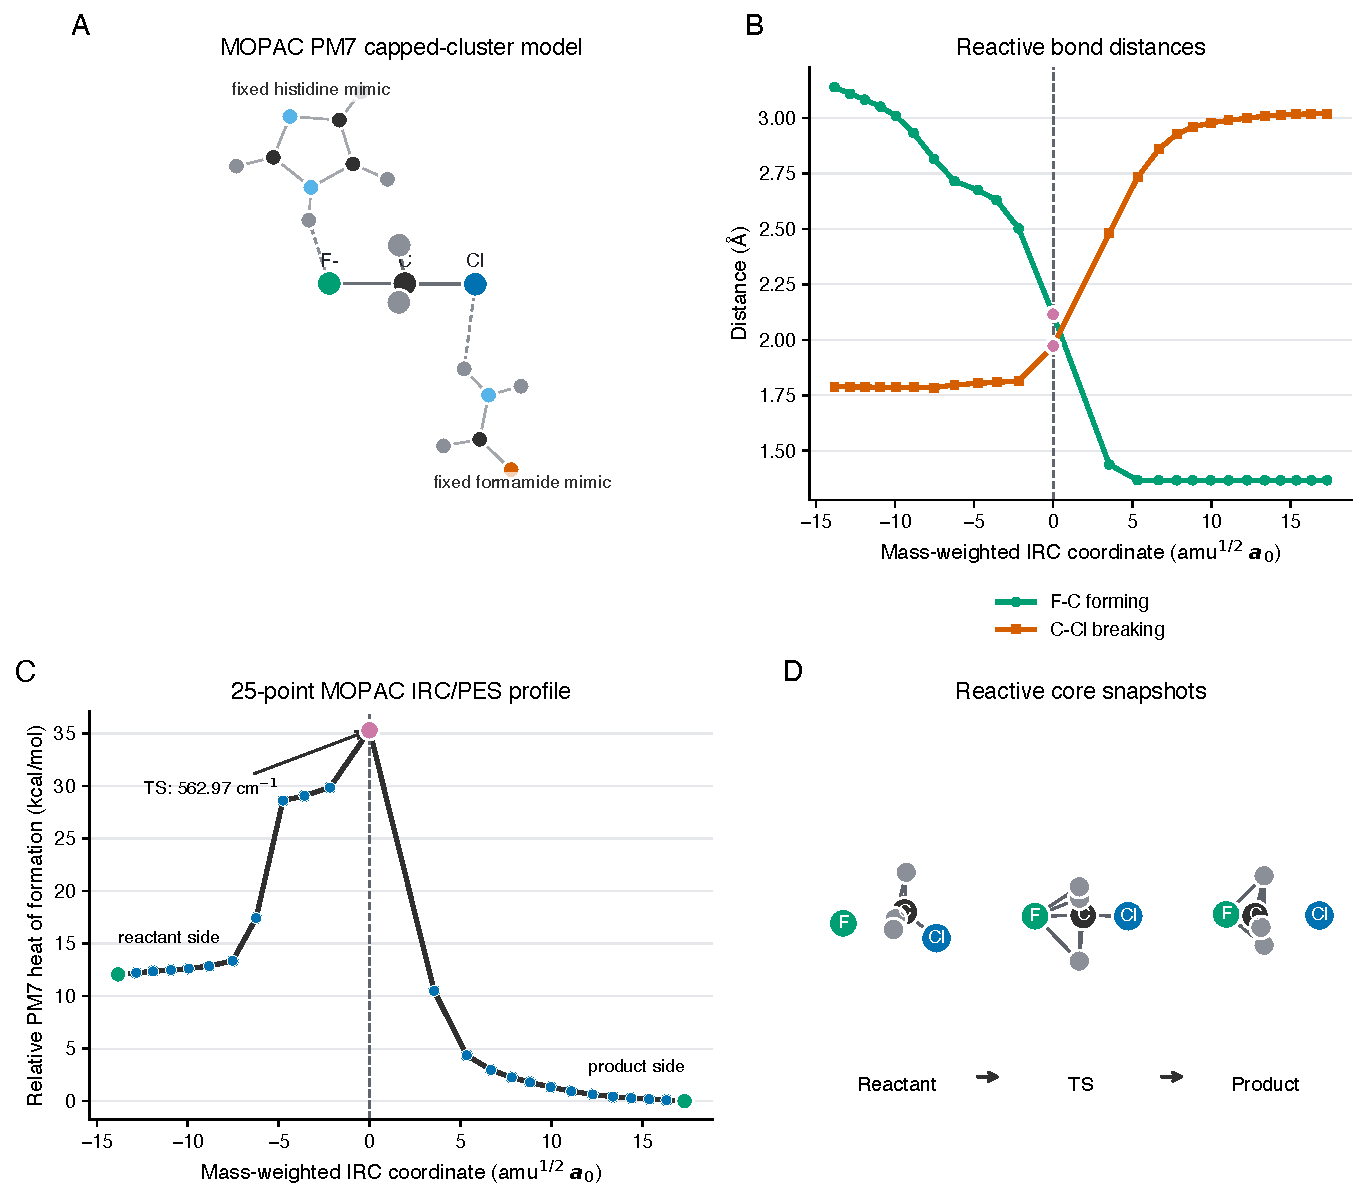
\includegraphics[width=\textwidth]{../figures/figure_8_mopac_capped_cluster_reaction.pdf}
\caption{MOPAC PM7 synthetic capped-cluster reaction-path example.  MOPAC provides the semiempirical PM7 energies and gradients, while Leonardo contributes the object mapping, QST-like workflow labeling, transition-state check and plotting layer \cite{mopac_joss2026,pm7_stewart2013,peng_schlegel_qst1993,gonzalez_schlegel_irc1990}.  (A) The 21-atom fixed capped-cluster model contains a reactive F$^-$/CH$_3$Cl core plus fixed histidine and formamide mimics.  (B) Forming F--C and breaking C--Cl distances change along the mass-weighted IRC coordinate.  (C) The selected QST3-like transition state has one dominant imaginary frequency and connects to a 25-point PM7 IRC/PES profile.  (D) Reactant-side, transition-state and product-side reactive-core snapshots are exported from the generated IRC XYZ trajectory.  This is a synthetic capped-cluster workflow demonstration, not a protein-derived QM/MM calculation or enzymatic-rate validation.}
\label{fig:mopaccluster}
\end{figure}

\begin{figure}[htbp]
\centering
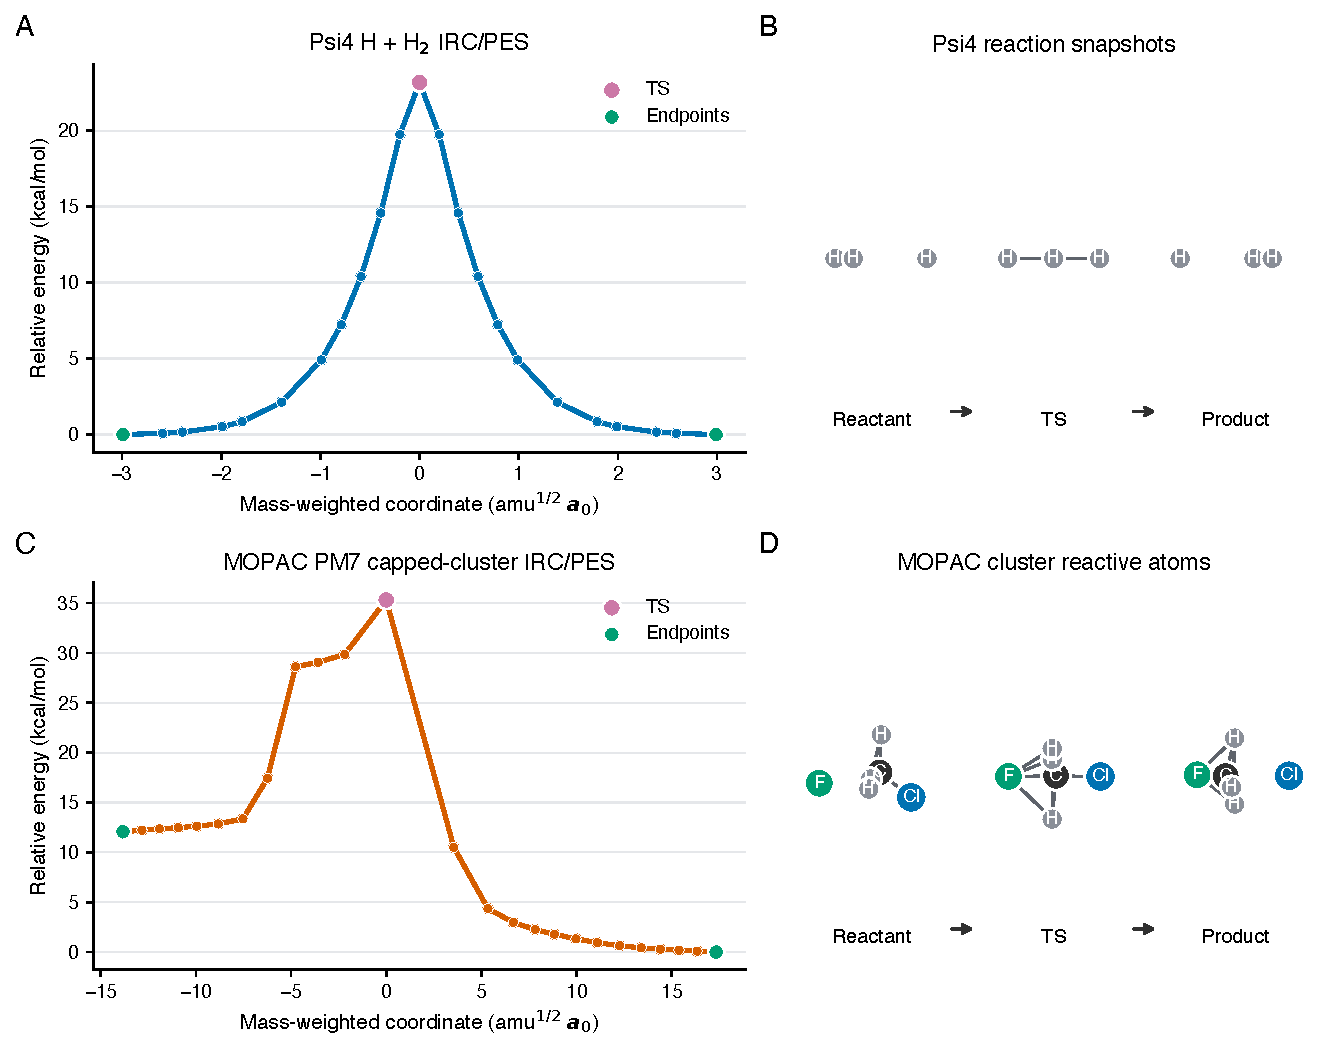
\includegraphics[width=\textwidth]{../figures/figure_9_qst_irc_reaction_paths.pdf}
\caption{Leonardo QST-like/IRC reaction-path workflow checks.  (A) Psi4 H + H$_2$ IRC/PES profile for a three-atom case.  (B) Psi4 reactant, transition-state and product snapshots from the generated IRC XYZ.  (C) MOPAC PM7 capped-cluster IRC/PES profile for a 21-atom case.  (D) MOPAC reactive atom snapshots for reactant, transition state and product.  Both examples use 25 IRC points and check Leonardo's workflow orchestration, parsing and plotting rather than general transition-state accuracy.}
\label{fig:qstirc}
\end{figure}

\section{Validation scope and limitations}\label{sec:limitations}

The workflow checks demonstrate that Leonardo can coordinate representative workflows and generate reproducible outputs, but they do not replace domain-specific benchmark studies for each scientific method.  The interaction-analysis example checks parsing, residue-level contact grouping and conservative charge-aware reporting on one protein-ligand structure; broader comparison against tools such as PLIP across diverse complexes is future work.  The pocket-docking example checks fpocket parsing, grid construction and smina pose-summary reporting, not pocket-detection or docking accuracy.  The redocking example uses a well-behaved streptavidin/biotin case and repeated seeds; it supports the template-mapping and RMSD-reporting workflow but does not constitute a multi-target docking benchmark.  The virtual-screening example checks ligand-library parsing and descriptor quality control, not enrichment performance, because no active/decoy benchmark set was included.

The OpenMM collective-variable example uses ACE-ALA-NME to exercise backend setup, metadynamics-style execution tracking and diagnostic-grid plotting on a compact molecule.  It supports the software claim that Leonardo can execute and visualize CV workflows, but it should not be interpreted as a biological protein-scale free-energy benchmark or an uncertainty-calibrated comparison of force fields.  Similarly, the guided-exit binding diagnostic is framed as a resource-limited workflow for preliminary studies; the 5 ns run checks guided-exit setup, trajectory analysis and state gating after both bound and unbound hold windows are populated.  Production absolute binding free energies still require system-specific convergence checks, careful restraints, repeated sampling, standard-state/restraint corrections and comparison with experimental or established computational references \cite{boresch_abfe2003,mey_alchemical2020}.  The Psi4 and MOPAC examples check atom mapping, transition-state checks and IRC plotting on compact systems.  The MOPAC example is a synthetic capped cluster with fixed histidine/formamide mimics, not a full protein-derived QM/MM calculation.  These limitations define the manuscript's claim: Leonardo provides an auditable structural-bioinformatics workflow layer around established engines, while scientific accuracy remains dependent on the selected engine, input preparation, sampling design and system-specific assessment.

\section{Conclusions}\label{sec:conclusions}

Leonardo provides a modular PyMOL-based platform for structural bioinformatics workflows that connect sequence analysis, structure preparation, protein-ligand interaction analysis, pocket docking, redocking, virtual screening, molecular dynamics, guided-exit binding diagnostics, quantum chemistry and semiempirical capped-cluster reaction-path analysis.  Its contribution is the transparent workflow layer: object-aware graphical setup, documented defaults, project tracking, testing, reporting and plotting around established scientific engines.  The evidence presented in this manuscript supports a software-platform claim focused on reproducible orchestration and backend verification; broader scientific benchmarks can be added module by module as community use cases expand.

\section*{List of abbreviations}

ABFE: absolute binding free energy; CV: collective variable; FES: free-energy surface; IRC: intrinsic reaction coordinate; MSA: multiple sequence alignment; PDB: Protein Data Bank; PES: potential-energy surface; QM/MM: quantum mechanics/molecular mechanics; QST: quadratic synchronous transit; RMSD: root-mean-square deviation; TS: transition state.

\section*{Availability and requirements}

\begin{itemize}
\item Project name: Leonardo.
\item Project home page: \url{https://github.com/juvenalyosa/Leonardo}.
\item Reviewer snapshot: GitHub tag \texttt{v0.2.0a2-reviewer}; a permanent public archive DOI remains pending for the exact journal-submission release.
\item Peer-review access: private GitHub repository \texttt{juvenalyosa/Leonardo}; reviewer access is provided by repository invitation while the project remains private.
\item Operating systems: workflow verification was performed on macOS; Linux installation scripts and environment specifications are distributed but still require clean-machine validation; Windows installation is provided through WSL2 helper scripts and remains pending independent validation.
\item Programming language: Python.
\item Installation: conda-based installation with an automated source-build and verification workflow.
\item Core requirements: PyMOL, Qt/PySide or PyQt, NumPy, Matplotlib, RDKit and Biopython.
\item Optional module-specific requirements: smina, fpocket, Meeko, Open Babel, AmberTools/OpenFF, OpenMM, PyMBAR, MDTraj, MODELLER, Psi4, MOPAC, AlphaFold/ColabFold, BLAST+, HMMER, MAFFT and Clustal Omega.
\item License: MIT for Leonardo source code.
\item Restrictions to use by non-academics: none under the Leonardo MIT license; third-party engines may have independent licenses, registration requirements or academic/commercial restrictions.
\end{itemize}

\section*{Declarations}

\subsection*{Ethics approval and consent to participate}

Not applicable.

\subsection*{Consent for publication}

Not applicable.

\subsection*{Availability of data and materials}

The source package, workflow-verification datasets, generated tables, test reports, figure-generation materials and checksum manifest are available in the private reviewer repository at \url{https://github.com/juvenalyosa/Leonardo}.  The reviewer snapshot is identified by GitHub tag \texttt{v0.2.0a2-reviewer}.  A permanent Zenodo DOI or equivalent archived release should be added for the exact public source package before journal submission.

\subsection*{Competing interests}

JY is affiliated with Protyon Tech.  MRG reports an external role as shareholder and CSO of Protyon BV.  AJvdW declares no competing interests.  The authors declare no other competing interests.

\subsection*{Funding}

The authors received no specific funding for this work.

\subsection*{Authors' contributions}

JY designed and implemented Leonardo, performed workflow-verification analyses, generated figures and wrote the manuscript.  MRG contributed structural-biology and protein-ligand-modeling guidance and reviewed the manuscript.  AJvdW contributed clinical and translational-oncology perspective and reviewed the manuscript.  All authors read and approved the final manuscript.

\subsection*{Acknowledgements}

The authors acknowledge the developers and maintainers of the open-source scientific software cited in this work.

\bibliography{references}

\end{document}
